% *** Authors should verify (and, if needed, correct) their LaTeX system  ***
% *** with the testflow diagnostic prior to trusting their LaTeX platform ***
% *** with production work. IEEE's font choices can trigger bugs that do  ***
% *** not appear when using other class files.                            ***
% The testflow support page is at:
% http://www.michaelshell.org/tex/testflow/


%%*************************************************************************
%% Legal Notice:
%% This code is offered as-is without any warranty either expressed or
%% implied; without even the implied warranty of MERCHANTABILITY or
%% FITNESS FOR A PARTICULAR PURPOSE!
%% User assumes all risk.
%% In no event shall IEEE or any contributor to this code be liable for
%% any damages or losses, including, but not limited to, incidental,
%% consequential, or any other damages, resulting from the use or misuse
%% of any information contained here.
%%
%% All comments are the opinions of their respective authors and are not
%% necessarily endorsed by the IEEE.
%%
%% This work is distributed under the LaTeX Project Public License (LPPL)
%% ( http://www.latex-project.org/ ) version 1.3, and may be freely used,
%% distributed and modified. A copy of the LPPL, version 1.3, is included
%% in the base LaTeX documentation of all distributions of LaTeX released
%% 2003/12/01 or later.
%% Retain all contribution notices and credits.
%% ** Modified files should be clearly indicated as such, including  **
%% ** renaming them and changing author support contact information. **
%%
%% File list of work: IEEEtran.cls, New_IEEEtran_how-to.pdf, bare_jrnl_new_sample4.tex,
%%*************************************************************************
\PassOptionsToPackage{unicode}{hyperref}
\PassOptionsToPackage{hyphens}{url}
\PassOptionsToPackage{dvipsnames,svgnames,x11names}{xcolor}
% Note that the a4paper option is mainly intended so that authors in
% countries using A4 can easily print to A4 and see how their papers will
% look in print - the typesetting of the document will not typically be
% affected with changes in paper size (but the bottom and side margins will).
% Use the testflow package mentioned above to verify correct handling of
% both paper sizes by the user's LaTeX system.
%
% Also note that the "draftcls" or "draftclsnofoot", not "draft", option
% should be used if it is desired that the figures are to be displayed in
% draft mode.
%
\documentclass[
  journal,
]{IEEEtran}%
% If IEEEtran.cls has not been installed into the LaTeX system files,
% manually specify the path to it like:
% \documentclass[journal]{../sty/IEEEtran}
\usepackage[cmex10]{amsmath}
\usepackage{amssymb}
\usepackage{iftex}
\ifPDFTeX
  \usepackage[T1]{fontenc}
  \usepackage[utf8]{inputenc}
  \usepackage{textcomp} % provide euro and other symbols
\else % if luatex or xetex
  \usepackage{unicode-math} % this also loads fontspec
  \defaultfontfeatures{Scale=MatchLowercase}
  \defaultfontfeatures[\rmfamily]{Ligatures=TeX,Scale=1}
\fi
%\usepackage{lmodern}
\ifPDFTeX\else
\fi
% Use upquote if available, for straight quotes in verbatim environments
\IfFileExists{upquote.sty}{\usepackage{upquote}}{}
\IfFileExists{microtype.sty}{% use microtype if available
  \usepackage[]{microtype}
  \UseMicrotypeSet[protrusion]{basicmath} % disable protrusion for tt fonts
}{}
\makeatletter
\parindent    1.0em
\ifCLASSOPTIONcompsoc
  \parindent    1.5em
\fi
\makeatother
\usepackage{xcolor}
\setlength{\emergencystretch}{3em} % prevent overfull lines

\setcounter{secnumdepth}{5}
% Make \paragraph and \subparagraph free-standing
\ifx\paragraph\undefined\else
  \let\oldparagraph\paragraph
  \renewcommand{\paragraph}[1]{\oldparagraph{#1}\mbox{}}
\fi
\ifx\subparagraph\undefined\else
  \let\oldsubparagraph\subparagraph
  \renewcommand{\subparagraph}[1]{\oldsubparagraph{#1}\mbox{}}
\fi


\providecommand{\tightlist}{%
  \setlength{\itemsep}{0pt}\setlength{\parskip}{0pt}}\usepackage{longtable,booktabs,array}
\usepackage{calc} % for calculating minipage widths
% Correct order of tables after \paragraph or \subparagraph
\usepackage{etoolbox}
\makeatletter
\patchcmd\longtable{\par}{\if@noskipsec\mbox{}\fi\par}{}{}
\makeatother
% Allow footnotes in longtable head/foot
\IfFileExists{footnotehyper.sty}{\usepackage{footnotehyper}}{\usepackage{footnote}}
\makesavenoteenv{longtable}
\usepackage{graphicx}
\makeatletter
\def\maxwidth{\ifdim\Gin@nat@width>\linewidth\linewidth\else\Gin@nat@width\fi}
\def\maxheight{\ifdim\Gin@nat@height>\textheight\textheight\else\Gin@nat@height\fi}
\makeatother
% Scale images if necessary, so that they will not overflow the page
% margins by default, and it is still possible to overwrite the defaults
% using explicit options in \includegraphics[width, height, ...]{}
\setkeys{Gin}{width=\maxwidth,height=\maxheight,keepaspectratio}
% Set default figure placement to htbp
\makeatletter
\def\fps@figure{htbp}
\makeatother
% definitions for citeproc citations
\NewDocumentCommand\citeproctext{}{}
\NewDocumentCommand\citeproc{mm}{%
  \begingroup\def\citeproctext{#2}\cite{#1}\endgroup}
\makeatletter
 % allow citations to break across lines
 \let\@cite@ofmt\@firstofone
 % avoid brackets around text for \cite:
 \def\@biblabel#1{}
 \def\@cite#1#2{{#1\if@tempswa , #2\fi}}
\makeatother
\newlength{\cslhangindent}
\setlength{\cslhangindent}{1.5em}
\newlength{\csllabelwidth}
\setlength{\csllabelwidth}{3em}
\newenvironment{CSLReferences}[2] % #1 hanging-indent, #2 entry-spacing
 {\begin{list}{}{%
  \setlength{\itemindent}{0pt}
  \setlength{\leftmargin}{0pt}
  \setlength{\parsep}{0pt}
  % turn on hanging indent if param 1 is 1
  \ifodd #1
   \setlength{\leftmargin}{\cslhangindent}
   \setlength{\itemindent}{-1\cslhangindent}
  \fi
  % set entry spacing
  \setlength{\itemsep}{#2\baselineskip}}}
 {\end{list}}
\usepackage{calc}
\newcommand{\CSLBlock}[1]{\hfill\break\parbox[t]{\linewidth}{\strut\ignorespaces#1\strut}}
\newcommand{\CSLLeftMargin}[1]{\parbox[t]{\csllabelwidth}{\strut#1\strut}}
\newcommand{\CSLRightInline}[1]{\parbox[t]{\linewidth - \csllabelwidth}{\strut#1\strut}}
\newcommand{\CSLIndent}[1]{\hspace{\cslhangindent}#1}

\usepackage{physics}
\usepackage[version=3]{mhchem}
\usepackage{orcidlink}
\usepackage{float}
\floatplacement{table}{htb}
\makeatletter
\@ifpackageloaded{caption}{}{\usepackage{caption}}
\AtBeginDocument{%
\ifdefined\contentsname
  \renewcommand*\contentsname{Table of contents}
\else
  \newcommand\contentsname{Table of contents}
\fi
\ifdefined\listfigurename
  \renewcommand*\listfigurename{List of Figures}
\else
  \newcommand\listfigurename{List of Figures}
\fi
\ifdefined\listtablename
  \renewcommand*\listtablename{List of Tables}
\else
  \newcommand\listtablename{List of Tables}
\fi
\ifdefined\figurename
  \renewcommand*\figurename{Fig.}
\else
  \newcommand\figurename{Fig.}
\fi
\ifdefined\tablename
  \renewcommand*\tablename{Table}
\else
  \newcommand\tablename{Table}
\fi
}
\@ifpackageloaded{float}{}{\usepackage{float}}
\floatstyle{ruled}
\@ifundefined{c@chapter}{\newfloat{codelisting}{h}{lop}}{\newfloat{codelisting}{h}{lop}[chapter]}
\floatname{codelisting}{Listing}
\newcommand*\listoflistings{\listof{codelisting}{List of Listings}}
\makeatother
\makeatletter
\makeatother
\makeatletter
\@ifpackageloaded{caption}{}{\usepackage{caption}}
\@ifpackageloaded{subcaption}{}{\usepackage{subcaption}}
\makeatother
\usepackage[skip=2pt,font=footnotesize]{caption}
%\captionsetup{format=myformat}
\makeatletter
%\setlength{\cslhangindent}{0pt plus .5pt}
\providecommand{\bibfont}{\footnotesize}
\let\CSLReferences@rig=\CSLReferences
\renewcommand{\CSLReferences}[2]{
\bibfont\settowidth\csllabelwidth{[999]}
\CSLReferences@rig{#1}{#2}
\vskip 0.3\baselineskip plus 0.1\baselineskip minus 0.1\baselineskip%
}
\makeatother
\ifLuaTeX
  \usepackage{selnolig}  % disable illegal ligatures
\fi
\IfFileExists{bookmark.sty}{\usepackage{bookmark}}{\usepackage{hyperref}}
\IfFileExists{xurl.sty}{\usepackage{xurl}}{} % add URL line breaks if available
\urlstyle{same} % disable monospaced font for URLs
\hypersetup{
  pdftitle={SVD Based Image Processing Applications},
  pdfauthor={Siju K S; Dr.Soman K.P},
  pdfkeywords={Singular Value Decomposition (SVD), Image
Processing, Image Compression, Image Denoising, Digital
Watermarking, Noise Filtering, Matrix Factorization, Rank
Approximation, Frobenius Norm, Energy Compaction, Digital
Forensics, Signal Processing, Adaptive Image Processing, Orthogonal
Subspaces},
  colorlinks=true,
  linkcolor={blue},
  filecolor={Maroon},
  citecolor={Blue},
  urlcolor={Blue},
  pdfcreator={LaTeX via pandoc}}

% *** Do not adjust lengths that control margins, column widths, etc. ***
% *** Do not use packages that alter fonts (such as pslatex).         ***
% There should be no need to do such things with IEEEtran.cls V1.6 and later.
% (Unless specifically asked to do so by the journal or conference you plan
% to submit to, of course. )


% correct bad hyphenation here
\hyphenation{op-tical net-works semi-conduc-tor}

%
% paper title
% can use linebreaks \\ within to get better formatting as desired
% Do not put math or special symbols in the title.
% paper title
% can use linebreaks \\ within to get better formatting as desired
% Do not put math or special symbols in the title.
\title{SVD Based Image Processing Applications}

\author{
\thanks{No funding is recieved for completion of this project work}
Siju K S\orcidlink{0009-0004-1983-5574},~\IEEEmembership{Member, ISTE}
and~Dr.Soman K.P%
\thanks{Siju K S is with School of Artificial Intelligence, Amrita
Vishwa Vidyapeetham, Coimbatore, 641 112 India%
  Corresponding author: siju.swamy@saintgits.org
}
\thanks{CEN}
%by-author.affiliations
\thanks{Dr.Soman K.P is with Professor \& Dean, Amrita School of
Artificial Intelligence%
}
%by-author.affiliations
\thanks{Template created June 23, 2023; revised
\texttt{r\ format(Sys.Date(),format=\textquotesingle{}\%B\ \%d,\ \%Y\textquotesingle{})}.}
}
\begin{document}

% The paper headers
\markboth{ASAI, October 2024}{Project Report}

% use for special paper notices

% make the title area
\maketitle

% As a general rule, do not put math, special symbols or citations
% in the abstract or keywords.
\begin{abstract}
This study investigates the application of Singular Value Decomposition
(SVD) as an effective mathematical framework for various image
processing tasks. SVD offers a unique decomposition approach, making it
suitable for applications like image compression, denoising, and
watermarking by enabling optimal rank approximations and noise
separation. The robustness of SVD in handling large matrices allows it
to capture key image characteristics, preserving essential features
while reducing data requirements. By leveraging SVD's ability to
separate data into dominant and subdominant subspaces, this research
demonstrates enhanced image compression, effective noise reduction, and
secure watermark embedding. Experimental results validate SVD's utility
in optimizing image storage, clarity, and fidelity, with potential
implications for advancing adaptive image processing techniques.
\end{abstract}
% Note that keywords are not normally used for peerreview papers.
\begin{IEEEkeywords}
Singular Value Decomposition (SVD), Image Processing, Image
Compression, Image Denoising, Digital Watermarking, Noise
Filtering, Matrix Factorization, Rank Approximation, Frobenius
Norm, Energy Compaction, Digital Forensics, Signal Processing, Adaptive
Image Processing, Orthogonal Subspaces
\end{IEEEkeywords}

% For peer review papers, you can put extra information on the cover
% page as needed:
% \ifCLASSOPTIONpeerreview
% \begin{center} \bfseries EDICS Category: 3-BBND \end{center}
% \fi
%
% For peerreview papers, this IEEEtran command inserts a page break and
% creates the second title. It will be ignored for other modes.
% \IEEEpeerreviewmaketitle


\section{Introduction}\label{introduction}

Linear Algebra based SVD is a powerful method to be used within the
realm of digital image processing. SVD decomposes a matrix in to three
constitutive matrices U, S, and V, thus making it possible to represent
an image using a fewer number of values
\citeproc{ref-moonen1992singular}{{[}1{]}}. This characteristic has
practical usage such as for image compression by keeping few singular
values in \(S\) matrix and stores the characteristics feature of the
image, hence reduce storage.

Researches suggested that It can be done if appropriate number of
singular values maintained and image can be compressed at higher ratio
with good quality The number of singular values kept (and thus the size
of the image to be compressed) is always not more (and often far less)
than the number of pixels in the original image. Thus, SVD turns out to
be a relatively strong technique for applications where a minimum number
of storage space and bandwidth is required to be preserved during
transmission of signals such as in satellite imagery, medical imaging
and photo enhancement.

Singular Value Decomposition (SVD) is a powerful mathematical technique
with a diverse range of applications in image processing. While its
capabilities are well-established, there remains untapped potential in
fully harnessing its versatility. This paper delves into the rich
properties of SVD and demonstrates how they can be leveraged across
various image processing tasks, such as compression, watermarking, and
quality assessment.

The study presents several key findings. First, the experiments validate
known but underutilized characteristics of Singular Value Decomposition
(SVD) in the context of image processing. This serves to aid ongoing
efforts aimed at enhancing the application of these SVD characteristics.
Second, the research identifies new trends and challenges faced in the
application of SVD for image processing. Some of these trends are
corroborated by experimental data, while others require additional
verification. Finally, this work lays the groundwork for future
investigations, highlighting promising avenues for further exploration
and development.

Overall, this paper offers a comprehensive examination of the rich
properties of Singular Value Decomposition (SVD) and its multifaceted
applications in the field of image processing. By shedding light on both
the established and emerging aspects of SVD, the study paves the way for
more efficient and innovative applications of this powerful mathematical
technique.

\section{Related works}\label{related-works}

Andrews and Patterson (1976) explored the significant role of Singular
Value Decomposition (SVD) techniques in the realm of digital image
processing, particularly for applications that demand high computational
power and precise imaging capabilities. Their work highlighted the
versatility of SVD methods, which are applicable not only to images but
also to broader representations of point spread functions (PSF) and
impulse responses. The authors framed these techniques as natural
extensions of linear filtering theory, thereby situating SVD within
established methodologies for image enhancement and restoration
\citeproc{ref-andrews1976singular}{{[}2{]}}.

Moonen et al.~(1992) expanded upon the established QR updating scheme by
introducing a more versatile and generally applicable method for
updating the Singular Value Decomposition (SVD). Their approach enhances
the QR updating technique by integrating a Jacobi-type SVD procedure.
This innovative combination allows for the effective restoration of an
acceptable approximation of the SVD after only a few SVD steps following
each QR update. The authors demonstrated that this method not only
maintains a comparable computational cost to that of traditional QR
updating but also significantly reduces the overall computational burden
associated with SVD updates. \citeproc{ref-moonen1992singular}{{[}1{]}}.

In their paper, Kakarala and Ogunbona (2001) introduced a novel
multiresolution form of Singular Value Decomposition (SVD) designed for
enhanced signal analysis and approximation. Recognizing the inherent
strengths of traditional SVD---specifically its optimal decorrelation
and subrank approximation properties---the authors expanded upon these
foundations by developing a multiresolution approach that maintains
linear computational complexity
\citeproc{ref-kakarala2001signal}{{[}3{]}}.

D Chandra (2002) introduced a novel watermarking technique- scaled
additive approach- for digital images that employs Singular Value
Decomposition (SVD) as a foundational method. The paper provides
comprehensive simulation results that showcase the robustness of this
SVD-based watermarking approach against various common image
degradations, underscoring its effectiveness in preserving watermark
integrity in challenging conditions
\citeproc{ref-chandra2002digital}{{[}4{]}}.

Sadek (2008) explored the increasing prominence of Singular Value
Decomposition (SVD) as a robust and reliable technique for orthogonal
matrix decomposition in the field of signal processing, particularly in
the context of watermarking and data hiding. The author highlighted the
fundamental properties of SVD, such as its conceptual clarity and
stability, which contribute to its growing popularity in various
applications In the realm of watermarking, many researchers have focused
on leveraging the singular values of host images to embed hidden
information. However, Sadek introduced a critical examination of these
SVD-based watermarking techniques by presenting a counterfeiting attack
specifically targeting the embedded watermark information within the
singular values. The study underscored the inherent vulnerabilities of
this class of watermarking methods, revealing how singular values can be
easily compromised through a broad spectrum of image processing
operations and deliberate attacks
\citeproc{ref-sadek2008blind}{{[}5{]}}.

Sadek (2012) explores the potential of Singular Value Decomposition
(SVD) as a transformative tool in the realm of image processing. The
paper presents a comprehensive experimental survey highlighting SVD's
efficacy across various imaging applications and proposed the perceptual
forensic approach in image watermarking. Recognizing SVD as an
attractive algebraic transform, Sadek emphasizes that its application in
image processing is still in its early stages despite its
well-documented advantageous properties
\citeproc{ref-sadek2012svd}{{[}6{]}}.

In their study, Kahu and Rahate (2013) investigated the application of
Singular Value Decomposition (SVD) as a technique for image compression,
emphasizing its effectiveness in expressing image data through a limited
number of eigenvectors determined by the image's dimensionality. They
highlighted the significance of psycho-visual redundancies inherent in
images, which enable compression without compromising the quality of the
visual output \citeproc{ref-kahu2013image}{{[}7{]}}.

\section{Introduction to Singular Value Decomposition
(SVD)}\label{introduction-to-singular-value-decomposition-svd}

In linear algebra, Singular Value Decomposition (SVD) is a fundamental
factorization technique for rectangular real or complex matrices. It
provides a structure similar to the diagonalization of symmetric or
Hermitian square matrices, utilizing eigenvectors as a basis. SVD is
particularly advantageous due to its stability and effectiveness,
allowing for decomposition into a set of linearly independent
components, each contributing uniquely to the matrix's structure.

For a digital image \(X\) of size \(M \times N\) (where \(M \geq N\)),
the SVD of \(X\) is represented as:

\[
X = U \Sigma V^T
\]

where \(U\) is an \(M \times M\) orthogonal matrix, \(V\) is an
\(N \times N\) orthogonal matrix, and \(\Sigma\) is an \(M \times N\)
diagonal matrix. The matrices \(U = [u_1, u_2, \ldots, u_m]\) and
\(V = [v_1, v_2, \ldots, v_n]\) contain the left and right singular
vectors of \(X\), respectively, and \(\Sigma\) holds the singular values
\(\sigma_i\) of \(X\) along its diagonal in descending order of
magnitude, with all off-diagonal elements set to zero.

In this setup, \(U\) and \(V\) are unitary orthogonal matrices, meaning
that each column vector has a unit norm and is orthogonal to others. The
singular values \(\sigma_i\) in \(\Sigma\) indicate the energy
contribution of each corresponding component, while each pair of
singular vectors from \(U\) and \(V\) defines the spatial orientation or
geometry of these components.

The left singular vectors (LSCs) of \(X\) are the eigenvectors of the
matrix \(X X^T\), while the right singular vectors (RSCs) are
eigenvectors of \(X^T X\). Each singular value represents the 2-norm of
its associated component, with the largest singular values capturing the
most significant patterns or features in the data. This property allows
SVD to effectively highlight essential image components while
suppressing noise or less critical features, making it ideal for
applications focused on key structural features in image processing
\citeproc{ref-andrews1976singular}{{[}2{]}}.

\section{SVD- A New Tool for Image
Processing}\label{svd--a-new-tool-for-image-processing}

Singular Value Decomposition (SVD) is a powerful and robust method for
orthogonal matrix decomposition, widely valued for its stability and
conceptual clarity. These attributes have led to its growing popularity
in signal processing, particularly in the domain of image processing. As
an algebraic transformation, SVD brings several advantageous properties
to imaging, which this section examines. While some of these properties
are well-utilized, others present opportunities for further exploration
and application.

Several key properties of SVD make it particularly useful in image
processing. These include maximum energy packing, efficient solutions to
least squares problems, calculation of matrix pseudo-inverses, and
multivariate analysis \citeproc{ref-strang2022introduction}{{[}8{]}}. An
essential feature of SVD is its relationship to matrix rank and its
ability to approximate matrices at a given rank. Digital images, often
represented as low-rank matrices, can be effectively described by a
limited number of eigenimages. This approach allows image signals to be
manipulated in two distinct subspaces
\citeproc{ref-kamm1998svd}{{[}9{]}}.

In the sections that follow, key hypotheses related to these properties
are proposed and validated. For completeness, the theoretical SVD
theorems relevant to these applications are summarized, followed by a
practical review of SVD properties with experimental demonstrations.

\subsection{SVD subspaces and
architecture}\label{svd-subspaces-and-architecture}

The SVD method effectively divides a matrix into two orthogonal
subspaces: the dominant and subdominant subspaces. This division
corresponds to a partitioning of the \(M\)-dimensional vector space,
separating primary signal components from secondary ones
\citeproc{ref-kamm1998svd}{{[}9{]}}. Such a property is particularly
advantageous in applications like noise filtering and digital
watermarking, where isolating signal elements from noise or embedding
data is crucial \citeproc{ref-sadek2012svd}{{[}6{]}}.

In the context of image processing, SVD architecture further highlights
its utility. For an image decomposed via SVD, each singular value (SV)
represents the luminance level of a specific image layer, while the
associated singular vectors (SCs) provide the geometric structure of
that layer. Generally, prominent image features align with eigenimages
associated with larger singular values, while smaller singular values
correspond to components associated with noise
\citeproc{ref-kahu2013image}{{[}7{]}}.

\subsection{PCA versus SVD}\label{pca-versus-svd}

Principal Component Analysis (PCA), also known as the Karhunen-Loève
Transform (KLT) or the Hotelling Transform, is a technique for computing
dominant vectors that represent a given dataset. PCA achieves an optimal
basis for minimum mean squared reconstruction of data and is
computationally based on the SVD of the data matrix or the eigenvalue
decomposition of the data covariance matrix. SVD is closely related to
the eigenvalue-eigenvector decomposition of a square matrix \(X\) into
\(V\Lambda V^T\), where \(V\) is orthogonal, and \(\Lambda\) is
diagonal. Notably, the matrices \(U\) and \(V\) in SVD correspond to
eigenvectors of \(XX^T\) and \(X^TX\), respectively. If \(X\) is
symmetric, the singular values of \(X\) are the absolute values of its
eigenvalues \citeproc{ref-deisenroth2020mathematics}{{[}10{]}}.

\subsection{SVD Multiresolution}\label{svd-multiresolution}

SVD is known for its maximum energy packing capability, making it
particularly useful for applications requiring multiresolution analysis.
This approach enables statistical characterization of images across
multiple resolutions, with SVD decomposing a matrix into orthogonal
components that allow optimal sub-rank approximations. The
multiresolution properties of SVD provide a framework to measure several
critical image characteristics at various resolutions, including
isotropy, sparsity of principal components, self-similarity under
scaling, and decomposition of mean squared error into meaningful
components \citeproc{ref-kakarala2001signal}{{[}3{]}}.

\subsection{SVD oriented energy}\label{svd-oriented-energy}

In SVD-based analysis of oriented energy, both the rank of the problem
and the signal space orientation are identifiable. SVD allows
decomposition into linearly independent components, each with its own
energy contribution. Represented as a linear combination of principal
components, SVD highlights dominant components that define the rank of
the observed system, with a few key components effectively capturing the
system's structure. The concept of oriented energy is beneficial for
separating signals from different sources or selecting signal subspaces
with maximal activity and integrity. Singular values in SVD represent
the square root of energy in the corresponding principal direction, with
the primary direction often aligned with the first singular vector
\(V_1\). Dominance accuracy can be measured by evaluating the
difference, or normalized difference, between the first two singular
values \citeproc{ref-sadek2008blind}{{[}5{]}}.

Many properties of SVD remain underutilized in image processing
applications. Subsequent sections will experimentally explore these
unexploited properties to demonstrate their potential for enhancing
various image processing techniques. Additional research is essential to
fully harness this versatile transformation in new and evolving
applications.

\section{Optimal Approximation and Noise Isolation Using
SVD}\label{optimal-approximation-and-noise-isolation-using-svd}

The SVD's unique ability to distinguish image content from noise is
critical for efficient matrix approximation. In an SVD-decomposed
matrix, the highest singular values capture the most essential
components of the image, while lower singular values represent noise. By
reconstructing the matrix with only the top \(k\) singular
values---forming an approximation \(X_k = U_k \Sigma_k V_k^T\)---SVD
yields an optimal representation that preserves primary image features
while suppressing noise. This characteristic makes SVD ideal for noise
filtering, compression, and forensic applications, where detectable
noise patterns are useful in watermarking and signal integrity
assessment. \#\#\# Rank approximation using SVD\}

Singular Value Decomposition (SVD) facilitates low-rank approximation,
enabling optimal sub-rank representations by emphasizing the largest
singular values that encapsulate the majority of the energy within an
image. SVD illustrates that a matrix can be expressed as a sum of
rank-one matrices. Given a matrix \(X \in \mathbb{R}^{m \times n}\) with
\(p = \min(m,n)\), the approximation can be represented as a truncated
matrix \(X_k\) with a specified rank \(k\). The representation is
formulated as follows:

\[
X \approx X_k = \sum_{i=1}^{k} s_i u_i v_i^T,
\]

where \(s_i\) are the singular values, \(u_i\) are the left singular
vectors, and \(v_i\) are the right singular vectors. Each term
\(s_i u_i v_i^T\) corresponds to a rank-one matrix, leading to the
conclusion that \(X\) is the sum of \(k\) rank-one matrices. This
approximation captures as much of the \emph{energy} of \(X\) as possible
while maintaining a rank of at most \(k\). Here, \emph{energy} is
quantified using the 2-norm or Frobenius norm.

The outer product \(u_i v_i^T\) results in a matrix of rank 1, requiring
\(M + N\) storage compared to \(M \times N\) for the original matrix.
For truncated SVD transformations with rank \(k\), the required storage
space is reduced to \((m+n+1)k\), demonstrating the efficiency of SVD in
applications such as image compression and watermarking.

\section{Example of SVD Application: Image
Reconstruction}\label{example-of-svd-application-image-reconstruction}

In this section, we demonstrate the application of Singular Value
Decomposition (SVD) on a JPEG image obtained from the internet. The
image is subjected to low-rank approximation using SVD to explore its
effectiveness in image reconstruction and compression.

For this experiment, we set the rank \(k = 40\). The original image,
denoted as \(X\), is decomposed into its singular values and singular
vectors as follows:

\[
X = U S V^T,
\]

where \(U\) is an orthogonal matrix containing the left singular
vectors, \(S\) is a diagonal matrix of singular values, and \(V^T\)
contains the right singular vectors. By retaining only the top \(k\)
singular values and their corresponding singular vectors, we can
reconstruct a low-rank approximation of the image:

\[
X_k \approx \sum_{i=1}^{k} s_i u_i v_i^T.
\]

In this instance, the low-rank approximation captures a significant
portion of the image's energy, effectively preserving the essential
visual features while reducing the noise and detail represented by the
higher-order singular values.

The reconstructed image using \(k = 40\) is displayed in
Fig.~\ref{fig-svdreconstruction}. This result illustrates the ability of
SVD to maintain the overall structure and key characteristics of the
original image while achieving a notable reduction in data size. The
efficiency of this low-rank approximation highlights the potential of
SVD for applications in image compression and restoration, allowing for
storage savings without substantial loss of quality.

This example underscores the practical utility of SVD in image
processing, offering a powerful tool for manipulating image data in
various applications, including compression, denoising, and feature
extraction.

\begin{figure}

\centering{

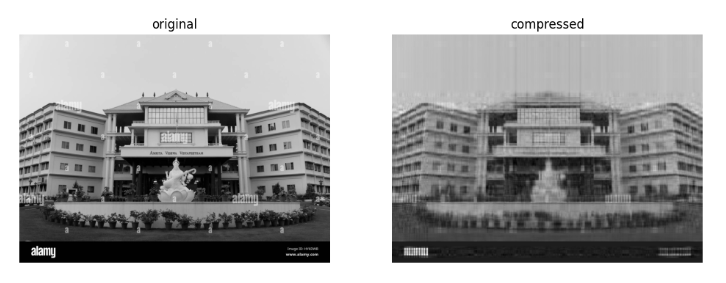
\includegraphics{./Notebooks/figures/SVD1.png}

}

\caption{\label{fig-svdreconstruction}Reconstructed image using SVD with
low-rank approximation (k=40).}

\end{figure}%

\section{Secrets of left and right singular
matrices}\label{secrets-of-left-and-right-singular-matrices}

The matrices \(U\) and \(V^T\) provide crucial insights into the
structural characteristics of the image, specifically the column space
and row space representations.

The left singular matrix \(U\) captures the column space of the image,
which represents the various features and patterns present in the image
across its vertical axis. In contrast, the right singular matrix \(V^T\)
captures the row space of the image, representing patterns across the
horizontal axis. By visualizing the first two components of these
matrices, we can reconstruct the primary patterns within the image
(refer Fig.~\ref{fig-SVD_components}).

The first two components of the column space from matrix \(U\) highlight
the dominant vertical patterns, while the first two components of the
row space from matrix \(V^T\) reveal the dominant horizontal patterns.
This reconstruction allows for a clear interpretation of how the image
is constructed from these fundamental features, showcasing the spatial
relationships inherent in the image data.

It is important to note that the components of \(V\) associated with the
smallest singular values correspond to noise in the image. This noise
resides in the null space of the image matrix \(X\) and contributes
minimally to the overall structure of the image. By identifying these
components, we can effectively distinguish between the essential
features of the image and the extraneous noise that may obscure its true
representation.

\begin{figure}

\centering{

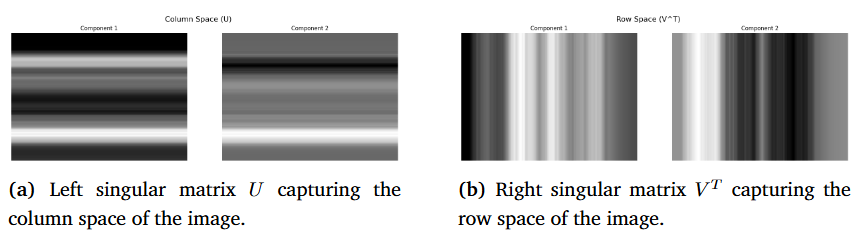
\includegraphics{./Notebooks/figures/SVDcomponents.png}

}

\caption{\label{fig-SVD_components}Visualization of the components
obtained from the SVD of the image.}

\end{figure}%

Figure {[}Fig.~\ref{fig-singular_value_distribution}\} displays the
log-mod distribution of the singular values from the SVD of the image,
providing insight into the energy contributions of each component.

\begin{figure}

\centering{

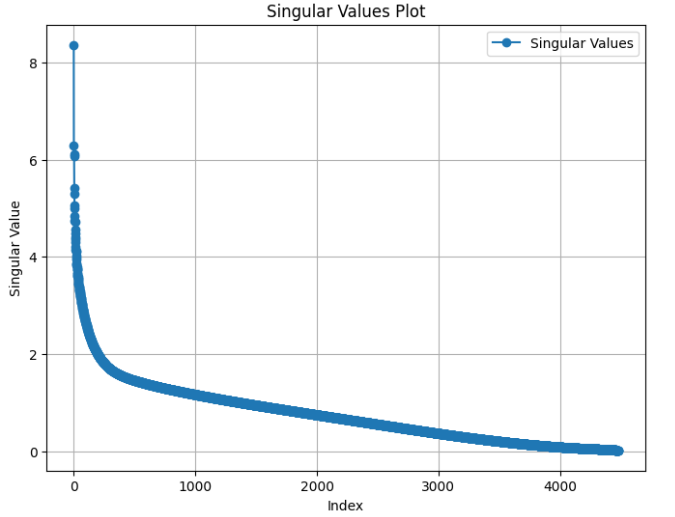
\includegraphics{./Notebooks/figures/singular-value-distribution.png}

}

\caption{\label{fig-singular_value_distribution}Distribution of the
singular values of the image.}

\end{figure}%

The log-mod distribution of the singular values reveals crucial
information about the image's structure and the underlying data's
dimensionality. The singular values, arranged in descending order,
represent the amount of energy each corresponding eigenimage contributes
to the overall image representation.

From Fig.~\ref{fig-singular_value_distribution}, a rapid decay in
singular values indicates that a small number of components capture the
majority of the image's energy, signifying a low-rank structure. This
property is advantageous for compression, as it suggests that the image
can be approximated using fewer outer products of rank-one matrices,
thus minimizing information loss.

The slope of the log-mod distribution further elucidates the
significance of each singular value; a steep drop-off signifies that
most information is concentrated in the first few singular values, while
the tail end, characterized by smaller singular values, is associated
with noise and less informative features of the image. This insight
allows for strategic selection of singular values in applications such
as compression and denoising, where retaining the dominant components
while discarding those associated with lower energy can enhance the
overall quality of the reconstructed image.

\subsection{Image quality metrics}\label{image-quality-metrics}

In the context of image compression and reconstruction using Singular
Value Decomposition (SVD), it is essential to evaluate the quality of
the reconstructed image. Three popular metrics for assessing image
quality are the Mean Squared Error (MSE), Peak Signal-to-Noise Ratio
(PSNR), and Structural Similarity Index Measure (SSIM). Each of these
metrics provides a different perspective on the quality of the
reconstructed image compared to the original.

\subsubsection{Mean Squared Error (MSE)}\label{mean-squared-error-mse}

The Mean Squared Error is a measure of the average squared differences
between the original and reconstructed images. It is defined
mathematically as:

\[
\text{MSE} = \frac{1}{N} \sum_{i=1}^{N} (I(i) - \hat{I}(i))^2
\]

where \(I(i)\) is the pixel value of the original image, \(\hat{I}(i)\)
is the pixel value of the reconstructed image, and \(N\) is the total
number of pixels in the image. Lower MSE values indicate better image
quality.

\subsubsection{Peak Signal-to-Noise Ratio
(PSNR)}\label{peak-signal-to-noise-ratio-psnr}

The Peak Signal-to-Noise Ratio is a logarithmic measure that compares
the maximum possible power of a signal to the power of corrupting noise
that affects the fidelity of its representation. It is given by:

\[
\text{PSNR} = 10 \cdot \log_{10} \left( \frac{\text{MAX}^2}{\text{MSE}} \right)
\] where \(\text{MAX}\) represents the maximum pixel value (e.g., 255
for 8-bit images). Higher PSNR values indicate better image quality, as
they correspond to lower MSE values. Higher PSNR values generally
indicate better quality of the reconstructed image.

\subsubsection{Structural Similarity Index Measure
(SSIM)}\label{structural-similarity-index-measure-ssim}

The Structural Similarity Index Measure assesses the visual impact of
three characteristics: luminance, contrast, and structure. The SSIM
index is defined as:

\[
\text{SSIM}(I, \hat{I}) = \frac{(2\mu_I \mu_{\hat{I}} + C_1)(2\sigma_{I\hat{I}} + C_2)}{(\mu_I^2 + \mu_{\hat{I}}^2 + C_1)(\sigma_I^2 + \sigma_{\hat{I}}^2 + C_2)}
\]

where \(\mu_I\) and \(\mu_{\hat{I}}\) are the average pixel values of
the original and reconstructed images, \(\sigma_I^2\) and
\(\sigma_{\hat{I}}^2\) are the variances, and \(\sigma_{I\hat{I}}\) is
the covariance. The constants \(C_1\) and \(C_2\) are small values added
for stability. SSIM values range from -1 to 1, with values closer to 1
indicating better similarity.

These metrics can effectively evaluate the quality of images
reconstructed through SVD compression, providing insights into how well
the compression process preserves the original image details.

\subsubsection{Comparison of image compression
methods}\label{comparison-of-image-compression-methods}

In this section, we compare the performance of different image
compression methods, specifically focusing on Singular Value
Decomposition (SVD), Discrete Cosine Transform (DCT), Wavelet Transform
(Haar), Fractal Compression, Run-Length Encoding (RLE), and Predictive
Coding. Each method has its unique characteristics and is suitable for
different types of image data. The evaluation metrics used for
comparison include Mean Squared Error (MSE), Peak Signal-to-Noise Ratio
(PSNR), and Structural Similarity Index Measure (SSIM). A brief
description of compression methods is given below.

\begin{itemize}
\item
  \emph{Singular Value Decomposition:} A linear algebra technique that
  decomposes a matrix into singular values and orthogonal matrices,
  providing efficient low-rank approximations suitable for image
  compression.
\item
  \emph{DCT (Discrete Cosine Transform:} Widely used in JPEG
  compression, DCT transforms image data into a frequency domain,
  allowing for the quantization and truncation of less significant
  frequencies to reduce file size while maintaining visual quality.
\item
  \emph{Wavelet (Haar Transform):} Utilizes wavelet functions to
  represent data at different scales and resolutions, allowing for both
  spatial and frequency localization, making it effective for
  compressing images with varying detail levels.
\item
  \emph{Fractal Compression:} This method relies on self-similarity in
  images and encodes them by identifying and representing repetitive
  patterns, which can lead to high compression ratios, especially for
  natural images.
\item
  \emph{RLE (Run-Length Encoding):} A lossless compression technique
  that replaces sequences of the same data value with a single value and
  a count, making it effective for images with large uniform areas.
\item
  \emph{Predictive Coding:} This approach predicts pixel values based on
  neighboring pixels and encodes the difference between the predicted
  and actual values, effectively reducing redundancy in the image data.
\end{itemize}

The performance metrics for each compression method are summarized in
Table~\ref{tbl-image_compression_comparison}.

\begin{longtable}[]{@{}llll@{}}
\caption{Comparison of Image Compression
Methods}\label{tbl-image_compression_comparison}\tabularnewline
\toprule\noalign{}
Method & MSE & PSNR (dB) & SSIM \\
\midrule\noalign{}
\endfirsthead
\toprule\noalign{}
Method & MSE & PSNR (dB) & SSIM \\
\midrule\noalign{}
\endhead
\bottomrule\noalign{}
\endlastfoot
SVD & 36.1802 & 32.5461 & 0.8247 \\
DCT & 107.6621 & 27.8102 & 0.8217 \\
Wavelet & 32.9375 & 32.9539 & 0.9582 \\
Fractal & 20.4741 & 35.0188 & 0.9320 \\
RLE & 0.0000 & inf & 1.0000 \\
Predictive & 107.2521 & 27.8267 & 0.5477 \\
\end{longtable}

The comparison of various image compression methods, as presented in
Table~\ref{tbl-image_compression_comparison}, highlights the promising
performance of Singular Value Decomposition (SVD) image compression. The
SVD method achieved a Mean Squared Error (MSE) of 36.1802, a Peak
Signal-to-Noise Ratio (PSNR) of 32.5461 dB, and a Structural Similarity
Index Measure (SSIM) of 0.8247. In terms of image quality, a PSNR value
above 30 dB is generally considered acceptable for high-quality image
reconstruction, and the SVD method meets this criterion. Similarly, the
SSIM score of 0.8247 indicates a relatively high level of structural
similarity, as values closer to 1.0 are preferred for maintaining
perceptual quality. These results suggest that SVD is a promising
approach for image compression, effectively balancing compression
efficiency with visual quality, particularly suitable for applications
that require efficient storage and satisfactory image fidelity.

\subsection{Orthogonal subspaces in
SVD}\label{orthogonal-subspaces-in-svd}

The Singular Value Decomposition (SVD) of the original data matrix \(X\)
enables its decomposition into two orthogonal subspaces: the
\emph{dominant subspace}, represented by the components \(US_kV^T\),
which corresponds to the signal information, and the \emph{subdominant
subspace}, represented by \(US_{n-k}V^T\), which captures the noise
components. This dual representation provides a clear delineation of the
image data into signal and noise, significantly enhancing our ability to
analyze and process the data effectively. This formalism can be
represented as in Figure Fig.~\ref{fig-dom-subdom}.

\begin{figure}

\centering{

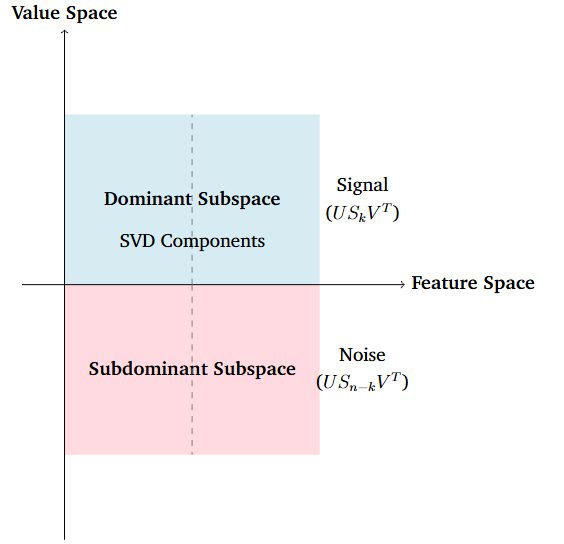
\includegraphics{./Notebooks/figures/domsubdom.png}

}

\caption{\label{fig-dom-subdom}Dominant-subdominant splitting of the
image SVD.}

\end{figure}%

Using the SVD, all the fundamental subspaces and their rank can be
extracted. This residing relationship can be visualized as:

\begin{align*}
  \mathbf{X} &=
  \mathbf{U} \, \Sigma \, \mathbf{V}^{T} \\
%
 &=
% U 
  \left[ \begin{array}{cc}
     \color{blue}{\mathbf{U}_{\mathcal{R}}} & \color{red}{\mathbf{U}_{\mathcal{N}}}
  \end{array} \right] 
  \left[ \begin{array}{cccc|cc}
     \sigma_{1} & 0 & \dots &  &   & \dots &  0 \\
     0 & \sigma_{2}  \\
     \vdots && \ddots \\
       & & & \sigma_{\rho} \\\hline
       & & & & 0 & \\
     \vdots &&&&&\ddots \\
     0 & & &   &   &  & 0 \\
  \end{array} \right]
  \left[ \begin{array}{c}
     \color{blue}{\mathbf{V}_{\mathcal{R}}}^{T} \\ 
     \color{red}{\mathbf{V}_{\mathcal{N}}}^{T}
  \end{array} \right]  \\
  & =
   \left[ \begin{array}{cccccccc}
    \color{blue}{u_{1}} & \dots & \color{blue}{u_{\rho}} & \color{red}{u_{\rho+1}} & \dots & \color{red}{u_{m}}
  \end{array} \right]
  \left[ \begin{array}{cc}
     \mathbf{S}_{\rho\times \rho} & \mathbf{0} \\
     \mathbf{0} & \mathbf{0} 
  \end{array} \right]
   \left[ \begin{array}{c}
    \color{blue}{v_{1}^{T}} \\ 
    \vdots \\
    \color{blue}{v_{\rho}^{T}} \\
    \color{red}{v_{\rho+1}^{T}} \\
    \vdots \\ 
    \color{red}{v_{n}^{T}}
  \end{array} \right]
\end{align*}

The column vectors form spans for the subspaces are given by

\begin{align*} 
% R A
\color{blue}{\mathcal{R} \left( \mathbf{X} \right)} &=
\text{span} \left\{
 \color{blue}{u_{1}}, \dots , \color{blue}{u_{\rho}}
\right\} \\
% R A*
\color{blue}{\mathcal{R} \left( \mathbf{X}^{T} \right)} &=
\text{span} \left\{
 \color{blue}{v_{1}}, \dots , \color{blue}{v_{\rho}}
\right\} \\
% N A*
\color{red}{\mathcal{N} \left( \mathbf{X}^{T} \right)} &=
\text{span} \left\{
\color{red}{u_{\rho+1}}, \dots , \color{red}{u_{m}}
\right\} \\
% N A
\color{red}{\mathcal{N} \left( \mathbf{X} \right)} &=
\text{span} \left\{
\color{red}{v_{\rho+1}}, \dots , \color{red}{v_{n}}
\right\} \\
%
\end{align*}

The conclusion is that the full SVD provides an orthonormal span for not
only the two null spaces, but also both range spaces. All these theories
can easily be extended to image processing. The right singular vectors
associated with the vanishing singular values of \(X\) define the null
space of the matrix, while the left singular vectors corresponding to
the non-zero singular values span the range of \(X\). Consequently, the
rank of \(X\) equals the count of non-zero singular values, which is
directly related to the number of non-zero diagonal elements in the
singular value matrix \(S\). This orthogonal partitioning of the
\(M\)-dimensional vector space mapped by \(X\) is essential in
applications such as image processing, where distinguishing between the
signal and noise components can significantly enhance techniques such as
watermarking.

Fig.~\ref{fig-svd-comparison} illustrates the image data's dominant
subspace, truncated to \(k = 50\) SVD components, alongside its
subdominant noise subspace.

\begin{figure}

\centering{

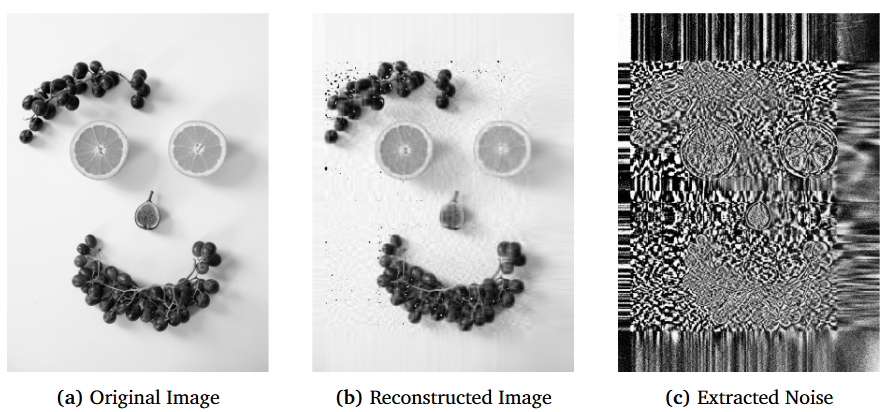
\includegraphics{./Notebooks/figures/svd_comparison.png}

}

\caption{\label{fig-svd-comparison}Comparison of Original Image,
Reconstructed Image after SVD Compression (with \(k=40\)), and Extracted
Noise. These subplots illustrate the effectiveness of SVD in
reconstructing the original image while isolating noise components.}

\end{figure}%

This property of SVD effectively facilitates the identification of the
rank of \(X\), the orthonormal basis for its range and null spaces, and
enables optimal low-rank approximations in various norms, thus paving
the way for significant advancements in image processing applications,
including watermarking, where the relationship between the SVD domain
and noisy or watermarked images can be leveraged effectively.

To investigate the influence of the truncation factor \(k\) on image
quality, experiments were conducted to evaluate the Peak Signal-to-Noise
Ratio (PSNR) and Structural Similarity Index (SSIM) values of
reconstructed images for various \(k\) values. The results, summarized
in Table~\ref{tbl-truncation_vs_quality}, indicate a clear trend: as the
truncation factor increases, both PSNR and SSIM improve significantly.
This improvement suggests that retaining more singular values enhances
the quality of the reconstructed images, thereby preserving essential
details and structures. Notably, the PSNR values reach a peak of 39.15
dB and the SSIM values approach 0.93 when \(k\) is set to 1000,
indicating high fidelity to the original image.

\begin{longtable}[]{@{}lll@{}}
\caption{Relationship between Truncation Factor \$k \$ and Image Quality
Metrics.}\label{tbl-truncation_vs_quality}\tabularnewline
\toprule\noalign{}
\(k\) & PSNR (dB) & SSIM \\
\midrule\noalign{}
\endfirsthead
\toprule\noalign{}
\(k\) & PSNR (dB) & SSIM \\
\midrule\noalign{}
\endhead
\bottomrule\noalign{}
\endlastfoot
1 & 14.445199 & 0.765134 \\
5 & 20.347972 & 0.779434 \\
10 & 22.906752 & 0.784555 \\
20 & 25.443104 & 0.789932 \\
50 & 28.667464 & 0.799783 \\
100 & 31.237551 & 0.814706 \\
200 & 33.401548 & 0.837690 \\
400 & 35.248494 & 0.870490 \\
600 & 36.602859 & 0.895303 \\
800 & 37.881342 & 0.915886 \\
1000 & 39.145403 & 0.933217 \\
\end{longtable}

Fig.~\ref{fig-psnr_ssim_variation_plot} illustrates the relationship
between the truncation factor \(k\) and the image quality metrics PSNR
and SSIM. The horizontal axis represents the truncation factor \(k\),
while the two curves depict the corresponding PSNR and SSIM values for
various \(k\) settings.

\begin{figure}

\centering{

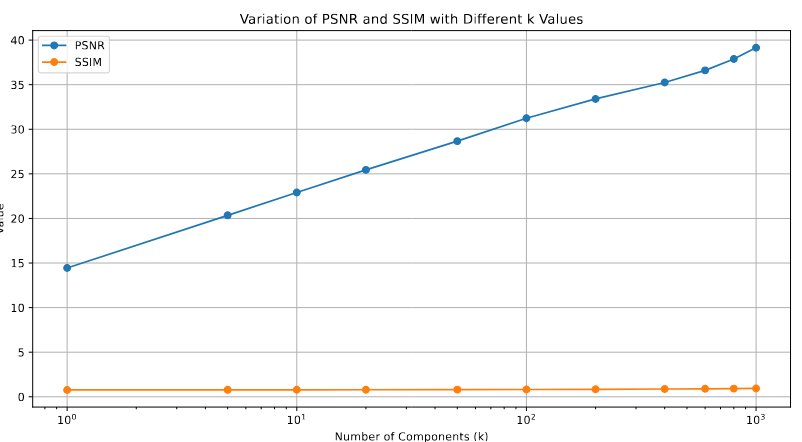
\includegraphics{./Notebooks/figures/psnr_ssim_variation_plot.png}

}

\caption{\label{fig-psnr_ssim_variation_plot}Variation of PSNR and SSIM
with respect to the truncation factor \$k \$.}

\end{figure}%

By analyzing the plot, one can easily determine the appropriate
truncation parameter \(k\) needed to achieve a desired PSNR or SSIM
value, thereby ensuring optimal fidelity and perceptual quality in the
reconstructed image. This graphical representation serves as a practical
tool for selecting the truncation factor, facilitating a balance between
compression efficiency and image quality. For instance, if a target PSNR
value of 35 dB is desired, one can project this value onto the PSNR
curve and trace down to the horizontal axis to identify the
corresponding \(k\) value, which allows for informed decision-making in
image compression settings.

\section{New Role- SVD as a Denoiser}\label{new-role--svd-as-a-denoiser}

Singular Value Decomposition (SVD) is a powerful mathematical technique
that has various applications in image processing, including noise
filtering and digital watermarking.

In the context of noise filtering, SVD can efficiently separate the
noise components from the original image signal. The SVD approximates
the image matrix by decomposing it into an optimal estimate of the
signal and the noise components. This property makes SVD a useful tool
for removing noise from images while preserving the quality and
recognition of the original content.

In this study, we assessed the correlation between consecutive
reconstructed images as a function of the truncation parameter \(k\) in
Singular Value Decomposition (SVD).

\begin{figure}

\centering{

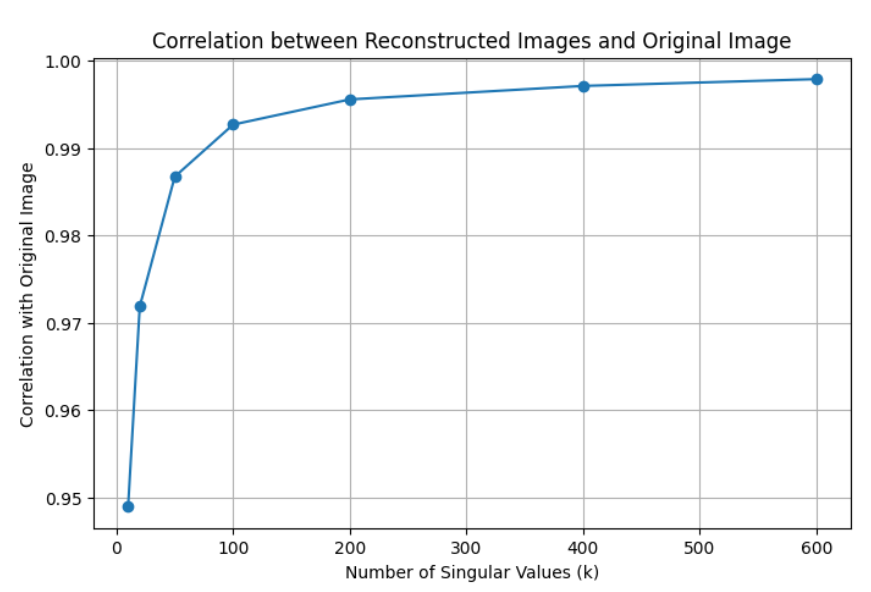
\includegraphics{./Notebooks/figures/corr-slice.png}

}

\caption{\label{fig-corr-slice}Correlation between original and
reconstructed images from image SVD.}

\end{figure}%

As shown in Fig.~\ref{fig-corr-slice}, the sharp increase in correlation
between consecutive reconstructed images as \(k\) rises to 200
illustrates SVD's strong ability to retain key image details even with
relatively low truncation levels. This trend suggests that the primary
singular values capture essential structural information of the original
image, leading to high-fidelity reconstructions while efficiently
filtering out less critical components. Given this preservation
capacity, we proceed to assess SVD's denoising capability by calculating
the PSNR and SSIM values for both the noisy and denoised images.

Fig.~\ref{fig-svd_denoising_results} illustrates experimental results of
the SVD-based denoising process on a high resolution image (20.0 MB,
\(4480\times 6133\), at 24 bit depth).

\begin{figure}

\centering{

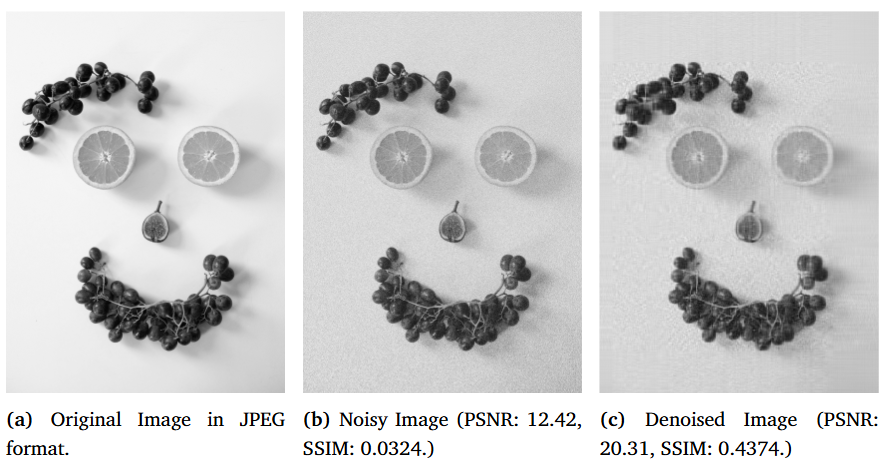
\includegraphics{./Notebooks/figures/svd_denoising_results.png}

}

\caption{\label{fig-svd_denoising_results}Comparison of Original, Noisy,
and Denoised Images using SVD.}

\end{figure}%

By considering the first 50 eigenimages as the image data subspace and
the remainder as the noise subspace, and then removing the noise
subspace, Fig.~\ref{fig-svd_denoising_results} (c) shows the image after
noise removal.

Noise has a disproportionate impact on singular values (SVs) and
singular vectors (SCs), with smaller SVs and their corresponding SCs
being more severely affected compared to larger SVs and SCs. Experiments
validate this phenomenon, as shown in
Fig.~\ref{fig-svd_matrices_comparison}, which depicts a 2-dimensional
representation of the left and right SCs. This highlights the contrast
between the slower changing waveforms of the former SCs and the faster
changing waveforms of the latter SCs.

\begin{figure}

\centering{

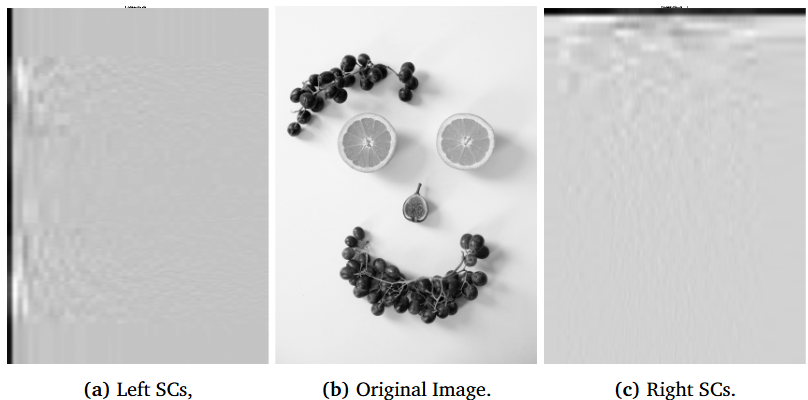
\includegraphics{./Notebooks/figures/svd_matrices_comparison.png}

}

\caption{\label{fig-svd_matrices_comparison}Comparison of the image with
the reconstructed traces in the left singular matrix (\(U\)) and the
right singular matrix (V\(^T\)) of noisy image.}

\end{figure}%

While SVD-based denoising methods have demonstrated promising results,
consistency in performance across different images is often challenging,
particularly within datasets like BSD400. In such cases, fixing a
truncation parameter \(k\) does not always yield optimal denoising
performance. This limitation arises because the variance of image
information captured in the singular values varies across different
images. Consequently, an adaptive approach is preferable over a fixed
truncation level for retaining significant image details while
effectively suppressing noise.

To address this, we propose dynamically thresholding the singular values
rather than fixing \(k\) for truncation. By removing singular values
below a specific threshold, we focus on preserving image components that
substantially contribute to the signal, thereby enhancing denoising
effectiveness. Experimentally, we observe that setting the truncation
threshold for singular values to \(0.618 \times \text{mean}(\Sigma)\),
where \(\Sigma\) denotes the diagonal matrix of singular values,
achieves optimal denoising. This threshold corresponds to approximately
61.8\% of the mean singular value magnitude, which is notably effective
in retaining essential image features while filtering out high-frequency
noise components.

Our empirical results further validate this approach, revealing that the
dynamic thresholding method consistently produces higher Peak
Signal-to-Noise Ratio (PSNR) values across a variety of images in the
BSD400 dataset when compared to fixed-\(k\) truncation. This improvement
underscores the robustness of the adaptive threshold in aligning the
denoising process with each image's inherent structural properties,
thereby achieving superior fidelity to the original image.

The effectiveness of the adaptive thresholding approach in Singular
Value Decomposition (SVD) for image denoising is exemplified in
Fig.~\ref{fig-svd_denoising_resultsBSD}. This figure displays an image
from the BSD400 dataset, showcasing the original, noisy input and
denoised output along with the PSNR and SSIM measures.

\begin{figure}

\centering{

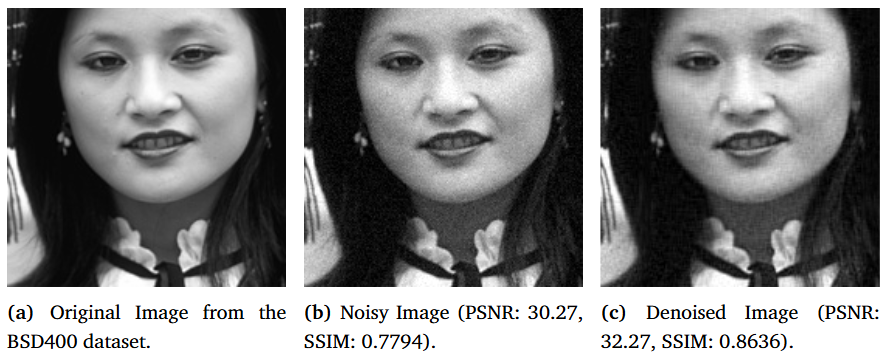
\includegraphics{./Notebooks/figures/svd_denoising_resultsBSD.png}

}

\caption{\label{fig-svd_denoising_resultsBSD}Comparison of Original,
Noisy, and Denoised images using SVD on BSD400 sample image.}

\end{figure}%

\subsection{Comparison and Advantages of SVD-Based Denoising in Medical
Imaging}\label{comparison-and-advantages-of-svd-based-denoising-in-medical-imaging}

In medical imaging, one major hurdle is the lack of a clean reference
image, which complicates the task of denoising. Creating datasets with
perfect reference images is often impossible. This challenge is made
even harder by the noise that arises from natural physiological
movements, which can introduce dynamic noise into MRI, CT, and
ultrasound scans, even if the patient is mostly still.

Many traditional denoising methods depend on machine learning algorithms
that are optimized with the help of reference images or alternative
\emph{doubly noisy} images that serve as substitutes for the ideal
ground truth. For example, recent research, including a study by Floquet
et al.~(2024), has shown that using noisy reference images can
effectively help adjust the parameters for denoising techniques.

In these scenarios, optimization methods such as the Scipy optimizer and
stochastic gradient optimization are applied to refine the algorithms,
aiming to reduce the Mean Square Error (MSE). This fine-tuning process
has resulted in impressive outcomes, achieving a Peak Signal-to-Noise
Ratio (PSNR) of 33.8, indicating a significant improvement in image
quality (reference:
\url{https://sijuswamy.github.io/Denoising-Manuscript/}).

On the other hand, an SVD-based approach has the potential to avoid the
requirement for having any ground truth reference which could be more
concept around it altogether. Using the SVD it is then possible to
filter noise depending on the singular values relating to structural
image information. The denoising based on SVD yielded a PSNR of 32.27 on
a similarly noisy image in a comparative experiment---a value with 5\%
from PSNRs achieved by parameter-optimized methods of denoising without
a need of a reference image. However, its independence from ground truth
is an advantage for medical applications where unsupervised methods may
reduce cost and complexity of operation.

These results could be further improved with a hybrid method that
combines a first stage of initial denoising and even using a noisy image
as a prior together with a method with optimized parameters then using
SVD to help capture dominant features in images. Even without a
reference image, SVD is able to act as an adaptive, standalone denoising
solution and opens sustainable possibilities in the medical innovations
context where the reference is commonly unknown and the denoising
process is crucial for the meaningful diagnosis.

\section{Image Forensics with SVD}\label{image-forensics-with-svd}

In the contemporary digital era, digital forensics has become crucial
for combating counterfeiting and manipulation of digital evidence aimed
at illicit profit or legal evasion. Forensic research encompasses
various domains, including steganography, watermarking, authentication,
and labeling. Numerous solutions have been developed to fulfill consumer
demands, such as authentication systems, DVD copy control, and
hardware/software watermarking.

Singular Value Decomposition (SVD) serves as a potent method in this
realm, concentrating significant signal energy into a minimal number of
coefficients while adapting to local statistical variations in images.
As an image-adaptive transform, SVD requires careful representation to
ensure accurate data retrieval.

\subsection{Image watermarking with scaled additive
approach}\label{image-watermarking-with-scaled-additive-approach}

SVD-based watermarking techniques exploit the stability of singular
values (SVs), which represent the image's luminance. Minor alterations
in these values do not drastically compromise the visual quality of the
host image. Methods typically utilize either the largest or smallest SVs
for watermark embedding, employing additive techniques or quantization.
For instance, D. Chandra's methodology involves the additive
incorporation of scaled watermark singular values into the singular
values of the host image \(X\)
\citeproc{ref-chandra2002digital}{{[}4{]}}:

\[
SV_{\text{modified}} = SV_{\text{original}} + \alpha \cdot \text{Watermark}
\]

Here, \(\alpha\) denotes a scaling factor, allowing for effective
watermark integration while maintaining the fidelity of the original
image. The scaled additive algorithm for image watermarking is given in
the following algorithm.

\phantomsection\label{algo-SA}
\textbf{Algorithm}: Scaled Additive Approach for Image Watermarking

\textbf{Inputs}: - Cover image \(A\) - Watermark \(W\) - Scaling factor
\(\alpha\)

\textbf{Outputs}: - Watermarked image \(A_w\) - Extracted watermark
\(W_e\)

\textbf{Steps}:

\begin{enumerate}
\def\labelenumi{\arabic{enumi}.}
\tightlist
\item
  \textbf{Watermark Embedding}:

  \begin{itemize}
  \tightlist
  \item
    Compute SVD of the cover image \(A\):
    \([U_1, S_1, V_1] \gets \text{svd}(A)\)
  \item
    Modify the singular values by adding the scaled watermark:
    \(\text{temp} \gets S_1 + (\alpha \cdot W)\)
  \item
    Compute SVD of the modified singular matrix:
    \([U_w, S_w, V_w] \gets \text{svd}(\text{temp})\)
  \item
    Reconstruct the watermarked image:
    \(A_w \gets U_1 \cdot S_w \cdot V_1^T\)
  \end{itemize}
\item
  \textbf{Watermark Extraction}:

  \begin{itemize}
  \tightlist
  \item
    Compute SVD of the watermarked image \(A_w\):
    \([U_{w1}, S_{w1}, V_{w1}] \gets \text{svd}(A_w)\)
  \item
    Reconstruct the matrix \(D\) using the new singular values:
    \(D \gets U_w \cdot S_{w1} \cdot V_w^T\)
  \item
    Extract the watermark: \(W_e \gets \frac{D - S_1}{\alpha}\)
  \end{itemize}
\item
  \textbf{Verification}:

  \begin{itemize}
  \tightlist
  \item
    If \(W == W_e\):

    \begin{itemize}
    \tightlist
    \item
      The image is \textbf{not attacked}.
    \end{itemize}
  \item
    Else:

    \begin{itemize}
    \tightlist
    \item
      The image has been \textbf{attacked}.
    \end{itemize}
  \end{itemize}
\end{enumerate}

Fig.~\ref{fig-inageforensic} represent the typical workflow of image
forensic.

\begin{figure}

\centering{

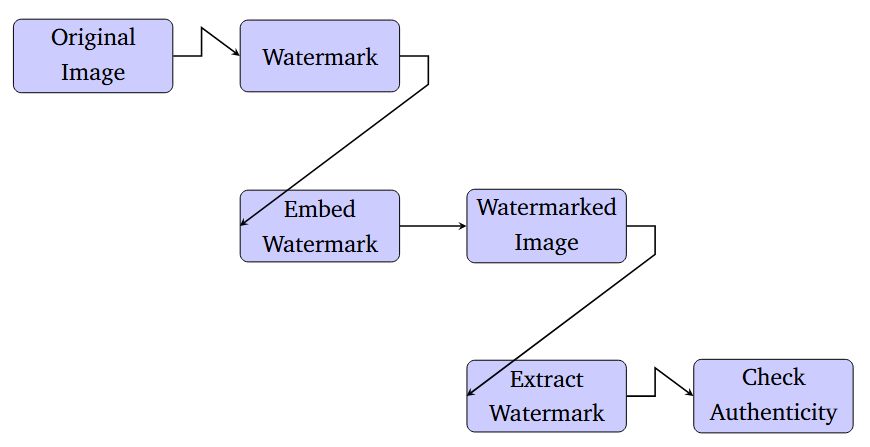
\includegraphics{./Notebooks/figures/inageforensic.png}

}

\caption{\label{fig-inageforensic}Image forensic workflow.}

\end{figure}%

Fig.~\ref{fig-image-forensicSVD} demonstrate the watermarking of images
using SVD. Since the extracted watermark is exactly what we embedded in
the covering image, no attack is detected
\citeproc{ref-Sharma2024}{{[}11{]}}.

\begin{figure}

\centering{

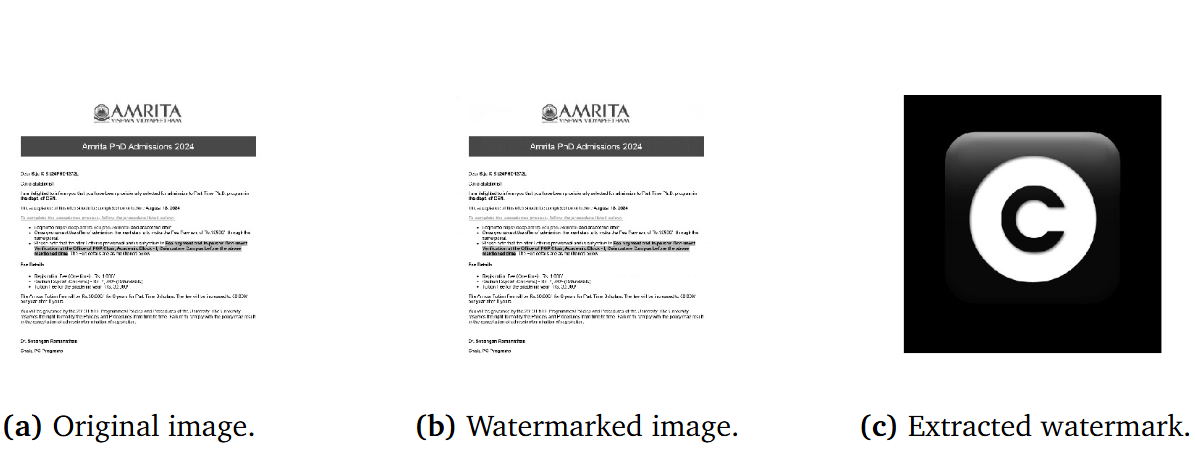
\includegraphics{./Notebooks/figures/image-forensicSVD.png}

}

\caption{\label{fig-image-forensicSVD}Demonstration of watermarking a
confidential image using SVD.}

\end{figure}%

In this first evaluation the PSNR value of watermarked image is 29.08
and the extraction is successful.

To evaluate the robustness and effectiveness of the Singular Value
Decomposition (SVD)-based watermarking approach on a broader spectrum of
images, using the BSD400 dataset offers a comprehensive test bed. The
BSD400 dataset contains a wide variety of images with intricate
textures, fine details, and different visual complexities, making it
ideal for testing how well the SVD-based watermarking technique can
embed and extract watermarks under varied conditions.

By selecting images with delicate content, such as running letters and
intricate textures, the goal is to assess how well the watermark remains
visually unobtrusive in complex scenes while being resilient to
potential attacks (such as noise, compression, or cropping). This method
will also allow for calculating objective quality metrics like PSNR
across different image categories, providing a robust understanding of
watermark quality and imperceptibility.

\subsection{Image watermarking with adaptive scaled additive
approach}\label{image-watermarking-with-adaptive-scaled-additive-approach}

Using the \emph{test\_077.png} image from the BSD400 dataset, we employ
an adaptive approach to watermarking that integrates D. Chandra's scaled
addition technique with a balanced formula
\citeproc{ref-chandra2002digital}{{[}4{]}}:

\begin{equation}
    \text{SV}_{\text{mod}} = (1 - \alpha) \cdot \text{SV}_{\text{img}} + \alpha \cdot \text{Watermark}
\end{equation}

Algorithm for the adaptive scaled additive (ASA) approach is shown
below.

\phantomsection\label{algo-ADAPTIVE}
\textbf{Algorithm}: Scaled Additive Adaptive Approach for Image
Watermarking

\textbf{Inputs}: - Cover image \(A\) - Watermark \(W\) - Scaling factor
\(\alpha\)

\textbf{Outputs}: - Watermarked image \(A_w\) - Extracted watermark
\(W_e\)

\textbf{Steps}:

\begin{enumerate}
\def\labelenumi{\arabic{enumi}.}
\tightlist
\item
  \textbf{Watermark Embedding}:

  \begin{itemize}
  \tightlist
  \item
    Compute SVD of the cover image \(A\):
    \([U_1, S_1, V_1] \gets \text{svd}(A)\)
  \item
    Modify the singular values by adding the scaled watermark
    adaptively:
    \(\text{temp} \gets (1 - \alpha) \cdot S_1 + (\alpha \cdot W)\)
  \item
    Compute SVD of the modified singular matrix:
    \([U_w, S_w, V_w] \gets \text{svd}(\text{temp})\)
  \item
    Reconstruct the watermarked image:
    \(A_w \gets U_1 \cdot S_w \cdot V_1^T\)
  \end{itemize}
\item
  \textbf{Watermark Extraction}:

  \begin{itemize}
  \tightlist
  \item
    Compute SVD of the watermarked image \(A_w\):
    \([U_{w1}, S_{w1}, V_{w1}] \gets \text{svd}(A_w)\)
  \item
    Reconstruct the matrix \(D\) using the new singular values:
    \(D \gets U_w \cdot S_{w1} \cdot V_w^T\)
  \item
    Extract the watermark: \(W_e \gets \frac{D - S_1}{\alpha}\)
  \end{itemize}
\item
  \textbf{Verification}:

  \begin{itemize}
  \tightlist
  \item
    If \(W == W_e\):

    \begin{itemize}
    \tightlist
    \item
      The image is \textbf{not attacked}.
    \end{itemize}
  \item
    Else:

    \begin{itemize}
    \tightlist
    \item
      The image has been \textbf{attacked}.
    \end{itemize}
  \end{itemize}
\end{enumerate}

This new approach modifies the singular values by proportionally
blending the image's original details with the watermark content based
on the parameter \(\alpha\). The adaptive blend allows for fine-tuning
the watermark's influence, thus optimizing both its visibility and
robustness.

This adaptive watermarking formula . The formula provides \emph{high
readability} and \emph{forensic resilience} and enables the watermark to
stay subtle within the image, while enhancing durability against
forensic attacks. This allows for improved image readability and detail
retention, particularly in face images like \emph{test\_077.png}.

As a next step, experiment with various values of \(\alpha\) to
fine-tune the watermark's visibility and robustness. Additionally,
evaluate the PSNR (Peak Signal-to-Noise Ratio) values to assess the
balance achieved by the adaptive method.

\subsection{Perceptual Forensic Approach for Image
Watermarking}\label{perceptual-forensic-approach-for-image-watermarking}

The perceptual forensic approach for image watermarking, introduced by
Sadek, represents a significant advance in singular value decomposition
(SVD)-based watermarking techniques by targeting robustness and
imperceptibility in forensic applications. This approach, termed Global
SVD (GSVD), employs a private (non-blind) methodology, making it
suitable for sensitive forensic tasks where watermark retrieval without
the original image is critical. In this technique, the watermark data is
optimally embedded within the host image's less significant subspace,
often referred to as the \emph{noise subspace}. This embedding choice
leverages the low-impact regions of the image's singular value
structure, thus maintaining the original image quality while preserving
the watermark's resilience.

A key innovation in Sadek's method is the scaled addition of the
watermark data subspace into the host image's singular values.
Traditional SVD-based watermarking techniques typically rely on a direct
scaled addition of watermark values to the singular values of the cover
image. However, this conventional approach often neglects the varying
magnitude across the singular value spectrum, leading to uneven
watermark integration that may affect image quality. Sadek's approach
addresses this limitation by \emph{flattening} the range of singular
values before watermark embedding, which smooths out the differences in
value magnitude and allows for a more perceptually consistent embedding.
This adjustment not only enhances the watermark's imperceptibility but
also strengthens its resilience against potential distortions or
attacks, which are common in forensic scenarios.

The GSVD-based perceptual forensic approach is inherently adaptable,
allowing the embedded watermark to withstand different types of image
manipulations depending on the robustness requirements. By embedding the
watermark within the less visually significant regions of the singular
value matrix, the GSVD technique achieves a balance between maintaining
high perceptual quality and ensuring the watermark's durability.

The algorithm for the perceptual forensic method for watermarking is
given below.

\phantomsection\label{algo-PFA}
\textbf{Algorithm}: Perceptual Forensic Watermarking using SVD

\textbf{Inputs}: - Cover image \(X\) - Watermark \(W\) - Scaling factor
\(\alpha\) - Threshold parameter \(k\)

\textbf{Outputs}: - Watermarked image \(Y\) - Extracted watermark
\(W_e\)

\textbf{Steps}:

\begin{enumerate}
\def\labelenumi{\arabic{enumi}.}
\item
  \textbf{Input}: Read cover image \(X\) and watermark \(W\).
\item
  \textbf{Compute SVD}: Perform the Singular Value Decomposition (SVD)
  on both \(X\) and \(W\):

  \begin{itemize}
  \tightlist
  \item
    \(X = U_h S_h V_h^T\)
  \item
    \(W = U_w S_w V_w^T\)
  \end{itemize}
\item
  \textbf{Define Scaled Addition for Modified Singular Values}:

  \begin{itemize}
  \tightlist
  \item
    For \(i = M - k\) to \(M\), with \(q = 1\) to \(k\):

    \begin{itemize}
    \tightlist
    \item
      \(S_m(i) = S_h(i) + \alpha \cdot \ln(S_w(q))\)
    \end{itemize}
  \item
    For all other \(i\), set \(S_m(i) = S_h(i)\).
  \end{itemize}
\item
  \textbf{Form the Watermarked Image} \(Y\):

  \begin{itemize}
  \tightlist
  \item
    \(Y = U_h S_m V_h^T\)
  \end{itemize}
\item
  \textbf{Reconstruct Singular Values for Watermark Extraction}:

  \begin{itemize}
  \tightlist
  \item
    For \(i = M - k\) to \(M\):

    \begin{itemize}
    \tightlist
    \item
      \(S'_w(i) = \exp\left(\frac{S_m(i) - S_h(i)}{\alpha}\right)\)
    \end{itemize}
  \end{itemize}
\item
  \textbf{Extract the Watermark}:

  \begin{itemize}
  \tightlist
  \item
    \(W_e = U_w S'_w V_w^T\)
  \end{itemize}
\item
  \textbf{Reconstruction Check}: Verify watermark accuracy by comparing
  \(W_e\) with \(W\).
\end{enumerate}

This method is particularly useful in forensic watermarking applications
that demand both high fidelity and robustness, such as in medical
imaging and high-resolution photographic forensics, where maintaining
image integrity is paramount. This technique's ability to fine-tune
watermark robustness based on singular value dynamics, while preserving
the host image quality, marks it as a promising advancement in forensic
watermarking applications.

Fig.~\ref{fig-perceptualplusscaledaddition} illustrate the results of
the adaptive watermarking technique using D. Chandra's approach and the
perceptual forensic approach, applied to a sample image in the BSD400
image dataset at \(\alpha=0.01\). The first row shows the original and
watermark-modified images, while the second row demonstrates the images
after the application of direct perceptual forensic watermarking and the
images with a Gaussian noise for forensic testing
\citeproc{ref-sadek2012svd}{{[}6{]}}.

\begin{figure}

\centering{

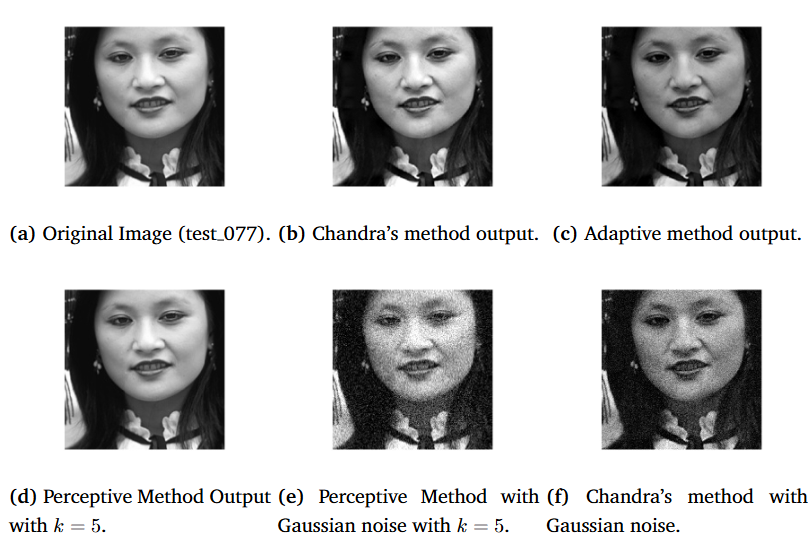
\includegraphics{./Notebooks/figures/perceptualplusscaledaddition.png}

}

\caption{\label{fig-perceptualplusscaledaddition}Results of Watermarking
with scaled addition and perceptual forensic approaches using SVD.}

\end{figure}%

From Fig.~\ref{fig-perceptualplusscaledaddition} (d), the perceptive
forensic approach is a winner in maintaining the image details in
watermarking and this fact is substantiated with Table~\ref{tbl-PSNRall}
. Also it is noted that noising after watermarking the image through SVD
produces almost same PSNR across the experiments. A detailed comparison
of image detailing after watermarking on uncompressed and compressed
version of the BSD400 image \emph{test\_077.png} is shown in Table
Table~\ref{tbl-PSNRcomparison}.

\begin{longtable}[]{@{}
  >{\raggedright\arraybackslash}p{(\columnwidth - 16\tabcolsep) * \real{0.1771}}
  >{\raggedright\arraybackslash}p{(\columnwidth - 16\tabcolsep) * \real{0.1042}}
  >{\raggedright\arraybackslash}p{(\columnwidth - 16\tabcolsep) * \real{0.1094}}
  >{\raggedright\arraybackslash}p{(\columnwidth - 16\tabcolsep) * \real{0.0990}}
  >{\raggedright\arraybackslash}p{(\columnwidth - 16\tabcolsep) * \real{0.1042}}
  >{\raggedright\arraybackslash}p{(\columnwidth - 16\tabcolsep) * \real{0.0990}}
  >{\raggedright\arraybackslash}p{(\columnwidth - 16\tabcolsep) * \real{0.1042}}
  >{\raggedright\arraybackslash}p{(\columnwidth - 16\tabcolsep) * \real{0.0990}}
  >{\raggedright\arraybackslash}p{(\columnwidth - 16\tabcolsep) * \real{0.1042}}@{}}
\caption{Peak Signal to Noise Ratio of various watermarked versions of
\emph{test\_077} image from BSD400 dataset under scaled additive (SA)
and adaptive scaled additive (ASA)
approaches.}\label{tbl-PSNRall}\tabularnewline
\toprule\noalign{}
\begin{minipage}[b]{\linewidth}\raggedright
Image type
\end{minipage} & \begin{minipage}[b]{\linewidth}\raggedright
\(\alpha=0.01\) (SA)
\end{minipage} & \begin{minipage}[b]{\linewidth}\raggedright
\(\alpha=0.01\) (ASA)
\end{minipage} & \begin{minipage}[b]{\linewidth}\raggedright
\(\alpha=0.1\) (SA)
\end{minipage} & \begin{minipage}[b]{\linewidth}\raggedright
\(\alpha=0.1\) (ASA)
\end{minipage} & \begin{minipage}[b]{\linewidth}\raggedright
\(\alpha=0.2\) (SA)
\end{minipage} & \begin{minipage}[b]{\linewidth}\raggedright
\(\alpha=0.2\) (ASA)
\end{minipage} & \begin{minipage}[b]{\linewidth}\raggedright
\(\alpha=0.3\) (SA)
\end{minipage} & \begin{minipage}[b]{\linewidth}\raggedright
\(\alpha=0.3\) (ASA)
\end{minipage} \\
\midrule\noalign{}
\endfirsthead
\toprule\noalign{}
\begin{minipage}[b]{\linewidth}\raggedright
Image type
\end{minipage} & \begin{minipage}[b]{\linewidth}\raggedright
\(\alpha=0.01\) (SA)
\end{minipage} & \begin{minipage}[b]{\linewidth}\raggedright
\(\alpha=0.01\) (ASA)
\end{minipage} & \begin{minipage}[b]{\linewidth}\raggedright
\(\alpha=0.1\) (SA)
\end{minipage} & \begin{minipage}[b]{\linewidth}\raggedright
\(\alpha=0.1\) (ASA)
\end{minipage} & \begin{minipage}[b]{\linewidth}\raggedright
\(\alpha=0.2\) (SA)
\end{minipage} & \begin{minipage}[b]{\linewidth}\raggedright
\(\alpha=0.2\) (ASA)
\end{minipage} & \begin{minipage}[b]{\linewidth}\raggedright
\(\alpha=0.3\) (SA)
\end{minipage} & \begin{minipage}[b]{\linewidth}\raggedright
\(\alpha=0.3\) (ASA)
\end{minipage} \\
\midrule\noalign{}
\endhead
\bottomrule\noalign{}
\endlastfoot
Watermarked & 61.84 & 46.41 & 38.83 & 26.56 & 30.82 & 20.68 & 25.16 &
17.35 \\
Noised after watermarked & 20.70 & 20.66 & 20.66 & 19.74 & 20.48 & 17.86
& 19.91 & 16.06 \\
Watermarked \& Compressed & 49.32 & 44.56 & 38.60 & 26.54 & 31.07 &
20.70 & 26.03 & 17.49 \\
\end{longtable}

From Table~\ref{tbl-PSNRcomparison}, it is clear that both scaled
additive and adaptive scaled additive approaches gives maximum image
detaining in the watermarked state is at lower values of \(\alpha\).
Maintaining readability and security is the key aspect in image
forensic. So \(\alpha=0.01\) is a safe choice. At the same level of
scaling the perceptual forensic approach is used in the BSD400 image.
Comparison of PSNR values of scaled additive, adaptive scaled additive
and the perceptual forensic approaches at \(\alpha=0.01\) is shown in
Table~\ref{tbl-PSNRall}.

\begin{longtable}[]{@{}
  >{\raggedright\arraybackslash}p{(\columnwidth - 6\tabcolsep) * \real{0.2329}}
  >{\raggedright\arraybackslash}p{(\columnwidth - 6\tabcolsep) * \real{0.2260}}
  >{\raggedright\arraybackslash}p{(\columnwidth - 6\tabcolsep) * \real{0.2877}}
  >{\raggedright\arraybackslash}p{(\columnwidth - 6\tabcolsep) * \real{0.2534}}@{}}
\caption{Peak Signal to Noise Ratio of various watermarked versions of
\emph{test\_077} image from BSD400 dataset under scaled additive (SA),
adaptive scaled additive (ASA) and perceptual forensic
approaches.}\label{tbl-PSNRcomparison}\tabularnewline
\toprule\noalign{}
\begin{minipage}[b]{\linewidth}\raggedright
Image type
\end{minipage} & \begin{minipage}[b]{\linewidth}\raggedright
Scaled Additive
\end{minipage} & \begin{minipage}[b]{\linewidth}\raggedright
Adaptive Scaled Additive
\end{minipage} & \begin{minipage}[b]{\linewidth}\raggedright
Perceptual Forensic
\end{minipage} \\
\midrule\noalign{}
\endfirsthead
\toprule\noalign{}
\begin{minipage}[b]{\linewidth}\raggedright
Image type
\end{minipage} & \begin{minipage}[b]{\linewidth}\raggedright
Scaled Additive
\end{minipage} & \begin{minipage}[b]{\linewidth}\raggedright
Adaptive Scaled Additive
\end{minipage} & \begin{minipage}[b]{\linewidth}\raggedright
Perceptual Forensic
\end{minipage} \\
\midrule\noalign{}
\endhead
\bottomrule\noalign{}
\endlastfoot
Watermarked & 61.84 & 46.41 & 75.17 \\
Noised after watermarked & 20.70 & 20.66 & 20.68 \\
Watermarked \& Compressed & 49.32 & 44.56 & 38.87 \\
\end{longtable}

Watermarking through Singular Value Decomposition (SVD) is emerging as a
promising method in the field of medical imaging to protect data
integrity and authenticity. In our study, an available CT image was used
to embed a watermark using both a scaled addition method and an adaptive
perceptual forensic approach.

When unaltered, the watermark was effectively extracted, showing that
SVD-based watermarking can preserve image integrity under normal
conditions. However, when noise was introduced after embedding, the
extracted watermark showed substantial degradation, highlighting the
technique's sensitivity to potential tampering.

\begin{figure}

\centering{

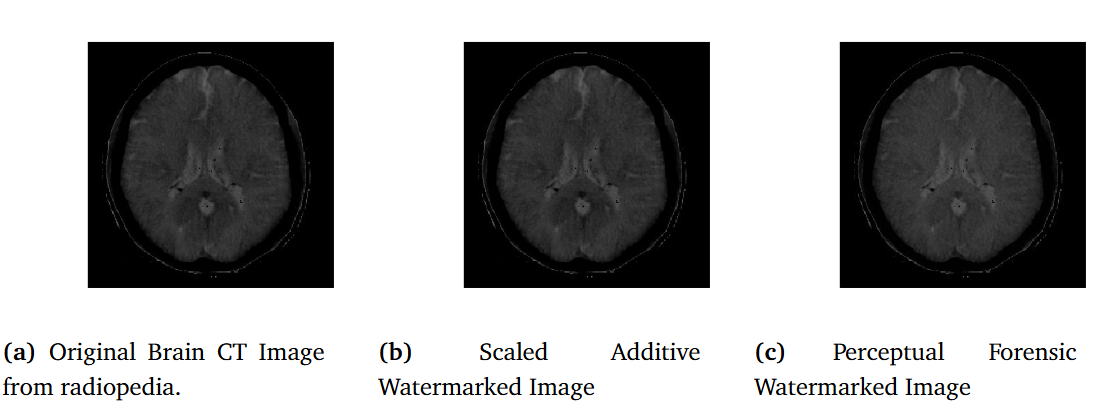
\includegraphics{./Notebooks/figures/BrainCTPerceptualWM.png}

}

\caption{\label{fig-BrainCTPerceptualWM}Comparison of Brain CT images:
(a) Original Brain CT Image, (b) Watermarked with scaled additive
approach, (c) Watermarked with perceptual forensic approach.}

\end{figure}%

The effect of watermarking on the Brain CT image using different image
forensic approaches is shown in Fig.~\ref{fig-BrainCTPerceptualWM}. The
scaled addition method achieved a Peak Signal-to-Noise Ratio (PSNR) of
33.93, balancing visibility and quality. Meanwhile, the perceptual
forensic approach, designed to better manage watermark strength relative
to image details, attained a PSNR of 102.87, maintaining high image
fidelity. These results indicate that SVD-based watermarking techniques
can be effective for medical imaging applications, where preserving
diagnostic quality while protecting image authenticity is critical. This
adaptive method offers a balanced approach to ensure data protection
without compromising readability and detail in medical images.

\section{Conclusion}\label{conclusion}

This study investigated SVD-based image processing applications,
specifically focusing on image compression, image denoising, and image
forensic analysis. Through experimental analysis on high-resolution
images, the BSD400 dataset, and medical images, this work examined the
effectiveness of two watermarking approaches: scaled additive embedding
and perceptual forensic embedding. In the scaled additive approach, the
watermark was scaled and embedded within the singular values of the
image before full SVD decomposition. To improve the adaptability across
images with varying detail levels, an adaptive scaling mechanism was
introduced, achieving high-quality image blending with minor scaling
factors \((\alpha < 0.02)\).

In the perceptual forensic approach, watermark embedding targeted
distinct ranges of singular values, optimizing the visibility and
robustness of the watermark under forensic scrutiny. This method
employed a locally adaptive SVD, enhancing watermark resilience while
preserving essential image details, making it effective for applications
requiring forensic analysis. Additionally, image denoising was
implemented as an automatic fine-tuning step to reduce noise introduced
during watermarking, further solidifying the watermark's readability and
stability.

This work is a partial replication and extension of Sadek's review on
SVD-based image processing applications, which highlights the
state-of-the-art methods and challenges in SVD applications for image
processing \citeproc{ref-sadek2012svd}{{[}6{]}}. By incorporating
aspects of automated fine-tuning for denoising algorithms in the
watermarking process, this study contributes a refined understanding of
how SVD can be leveraged to balance image quality and watermark
resilience. Overall, the findings affirm that SVD-based techniques
fulfill the study's objectives across compression, denoising, and
forensic applications, providing a flexible and robust approach to image
processing that is effective across various image types and contexts.
Future work may explore additional fine-tuning and new methodologies to
enhance forensic robustness and adaptive capabilities in real-world
applications.

\section{References}\label{references}

\phantomsection\label{refs}
\begin{CSLReferences}{0}{0}
\bibitem[\citeproctext]{ref-moonen1992singular}
\CSLLeftMargin{{[}1{]} }%
\CSLRightInline{M. Moonen, P. Van Dooren, and J. Vandewalle, {``A
singular value decomposition updating algorithm for subspace
tracking,''} \emph{SIAM Journal on Matrix Analysis and Applications},
vol. 13, no. 4, pp. 1015--1038, 1992. }

\bibitem[\citeproctext]{ref-andrews1976singular}
\CSLLeftMargin{{[}2{]} }%
\CSLRightInline{H. Andrews and C. Patterson, {``Singular value
decompositions and digital image processing,''} \emph{IEEE Transactions
on Acoustics, Speech, and Signal Processing}, vol. 24, no. 1, pp.
26--53, 1976. }

\bibitem[\citeproctext]{ref-kakarala2001signal}
\CSLLeftMargin{{[}3{]} }%
\CSLRightInline{R. Kakarala and P. O. Ogunbona, {``Signal analysis using
a multiresolution form of the singular value decomposition,''}
\emph{IEEE Transactions on Image processing}, vol. 10, no. 5, pp.
724--735, 2001. }

\bibitem[\citeproctext]{ref-chandra2002digital}
\CSLLeftMargin{{[}4{]} }%
\CSLRightInline{D. S. Chandra, {``Digital image watermarking using
singular value decomposition,''} in \emph{The 2002 45th midwest
symposium on circuits and systems, 2002. MWSCAS-2002.}, 2002, vol. 3,
pp. III--III. }

\bibitem[\citeproctext]{ref-sadek2008blind}
\CSLLeftMargin{{[}5{]} }%
\CSLRightInline{R. A. Sadek, {``{Blind synthesis attack on SVD based
watermarking techniques},''} in \emph{2008 international conference on
computational intelligence for modelling control \& automation}, 2008,
pp. 140--145. }

\bibitem[\citeproctext]{ref-sadek2012svd}
\CSLLeftMargin{{[}6{]} }%
\CSLRightInline{R. A. Sadek, {``{SVD based image processing
applications: state of the art, contributions and research
challenges},''} \emph{arXiv preprint arXiv:1211.7102}, 2012. }

\bibitem[\citeproctext]{ref-kahu2013image}
\CSLLeftMargin{{[}7{]} }%
\CSLRightInline{S. Kahu and R. Rahate, {``Image compression using
singular value decomposition,''} \emph{International Journal of
Advancements in Research \& Technology}, vol. 2, no. 8, pp. 244--248,
2013. }

\bibitem[\citeproctext]{ref-strang2022introduction}
\CSLLeftMargin{{[}8{]} }%
\CSLRightInline{G. Strang, \emph{Introduction to linear algebra}. SIAM,
2022. }

\bibitem[\citeproctext]{ref-kamm1998svd}
\CSLLeftMargin{{[}9{]} }%
\CSLRightInline{J. L. Kamm, {``{SVD-based methods for signal and image
restoration},''} \emph{PhD Thesis}, 1998. }

\bibitem[\citeproctext]{ref-deisenroth2020mathematics}
\CSLLeftMargin{{[}10{]} }%
\CSLRightInline{M. P. Deisenroth, A. A. Faisal, and C. S. Ong,
\emph{Mathematics for machine learning}. Cambridge University Press,
2020. }

\bibitem[\citeproctext]{ref-Sharma2024}
\CSLLeftMargin{{[}11{]} }%
\CSLRightInline{N. K. Sharma, {``{SVD Domain Watermarking}.''} 2024
{[}Online{]}. Available:
\url{https://www.mathworks.com/matlabcentral/fileexchange/64554-svd-domain-watermarking}}

\end{CSLReferences}


% Can use something like this to put references on a page
% by themselves when using endfloat and the captionsoff option.
\ifCLASSOPTIONcaptionsoff
  \newpage
\fi

% trigger a \newpage just before the given reference
% number - used to balance the columns on the last page
% adjust value as needed - may need to be readjusted if
% the document is modified later
%\IEEEtriggeratref{8}
% The "triggered" command can be changed if desired:
%\IEEEtriggercmd{\enlargethispage{-5in}}

% Uncomment when use biblatex with style=ieee
%\renewcommand{\bibfont}{\footnotesize} % for IEEE bibfont size

\pagebreak[3]
\begin{IEEEbiography}[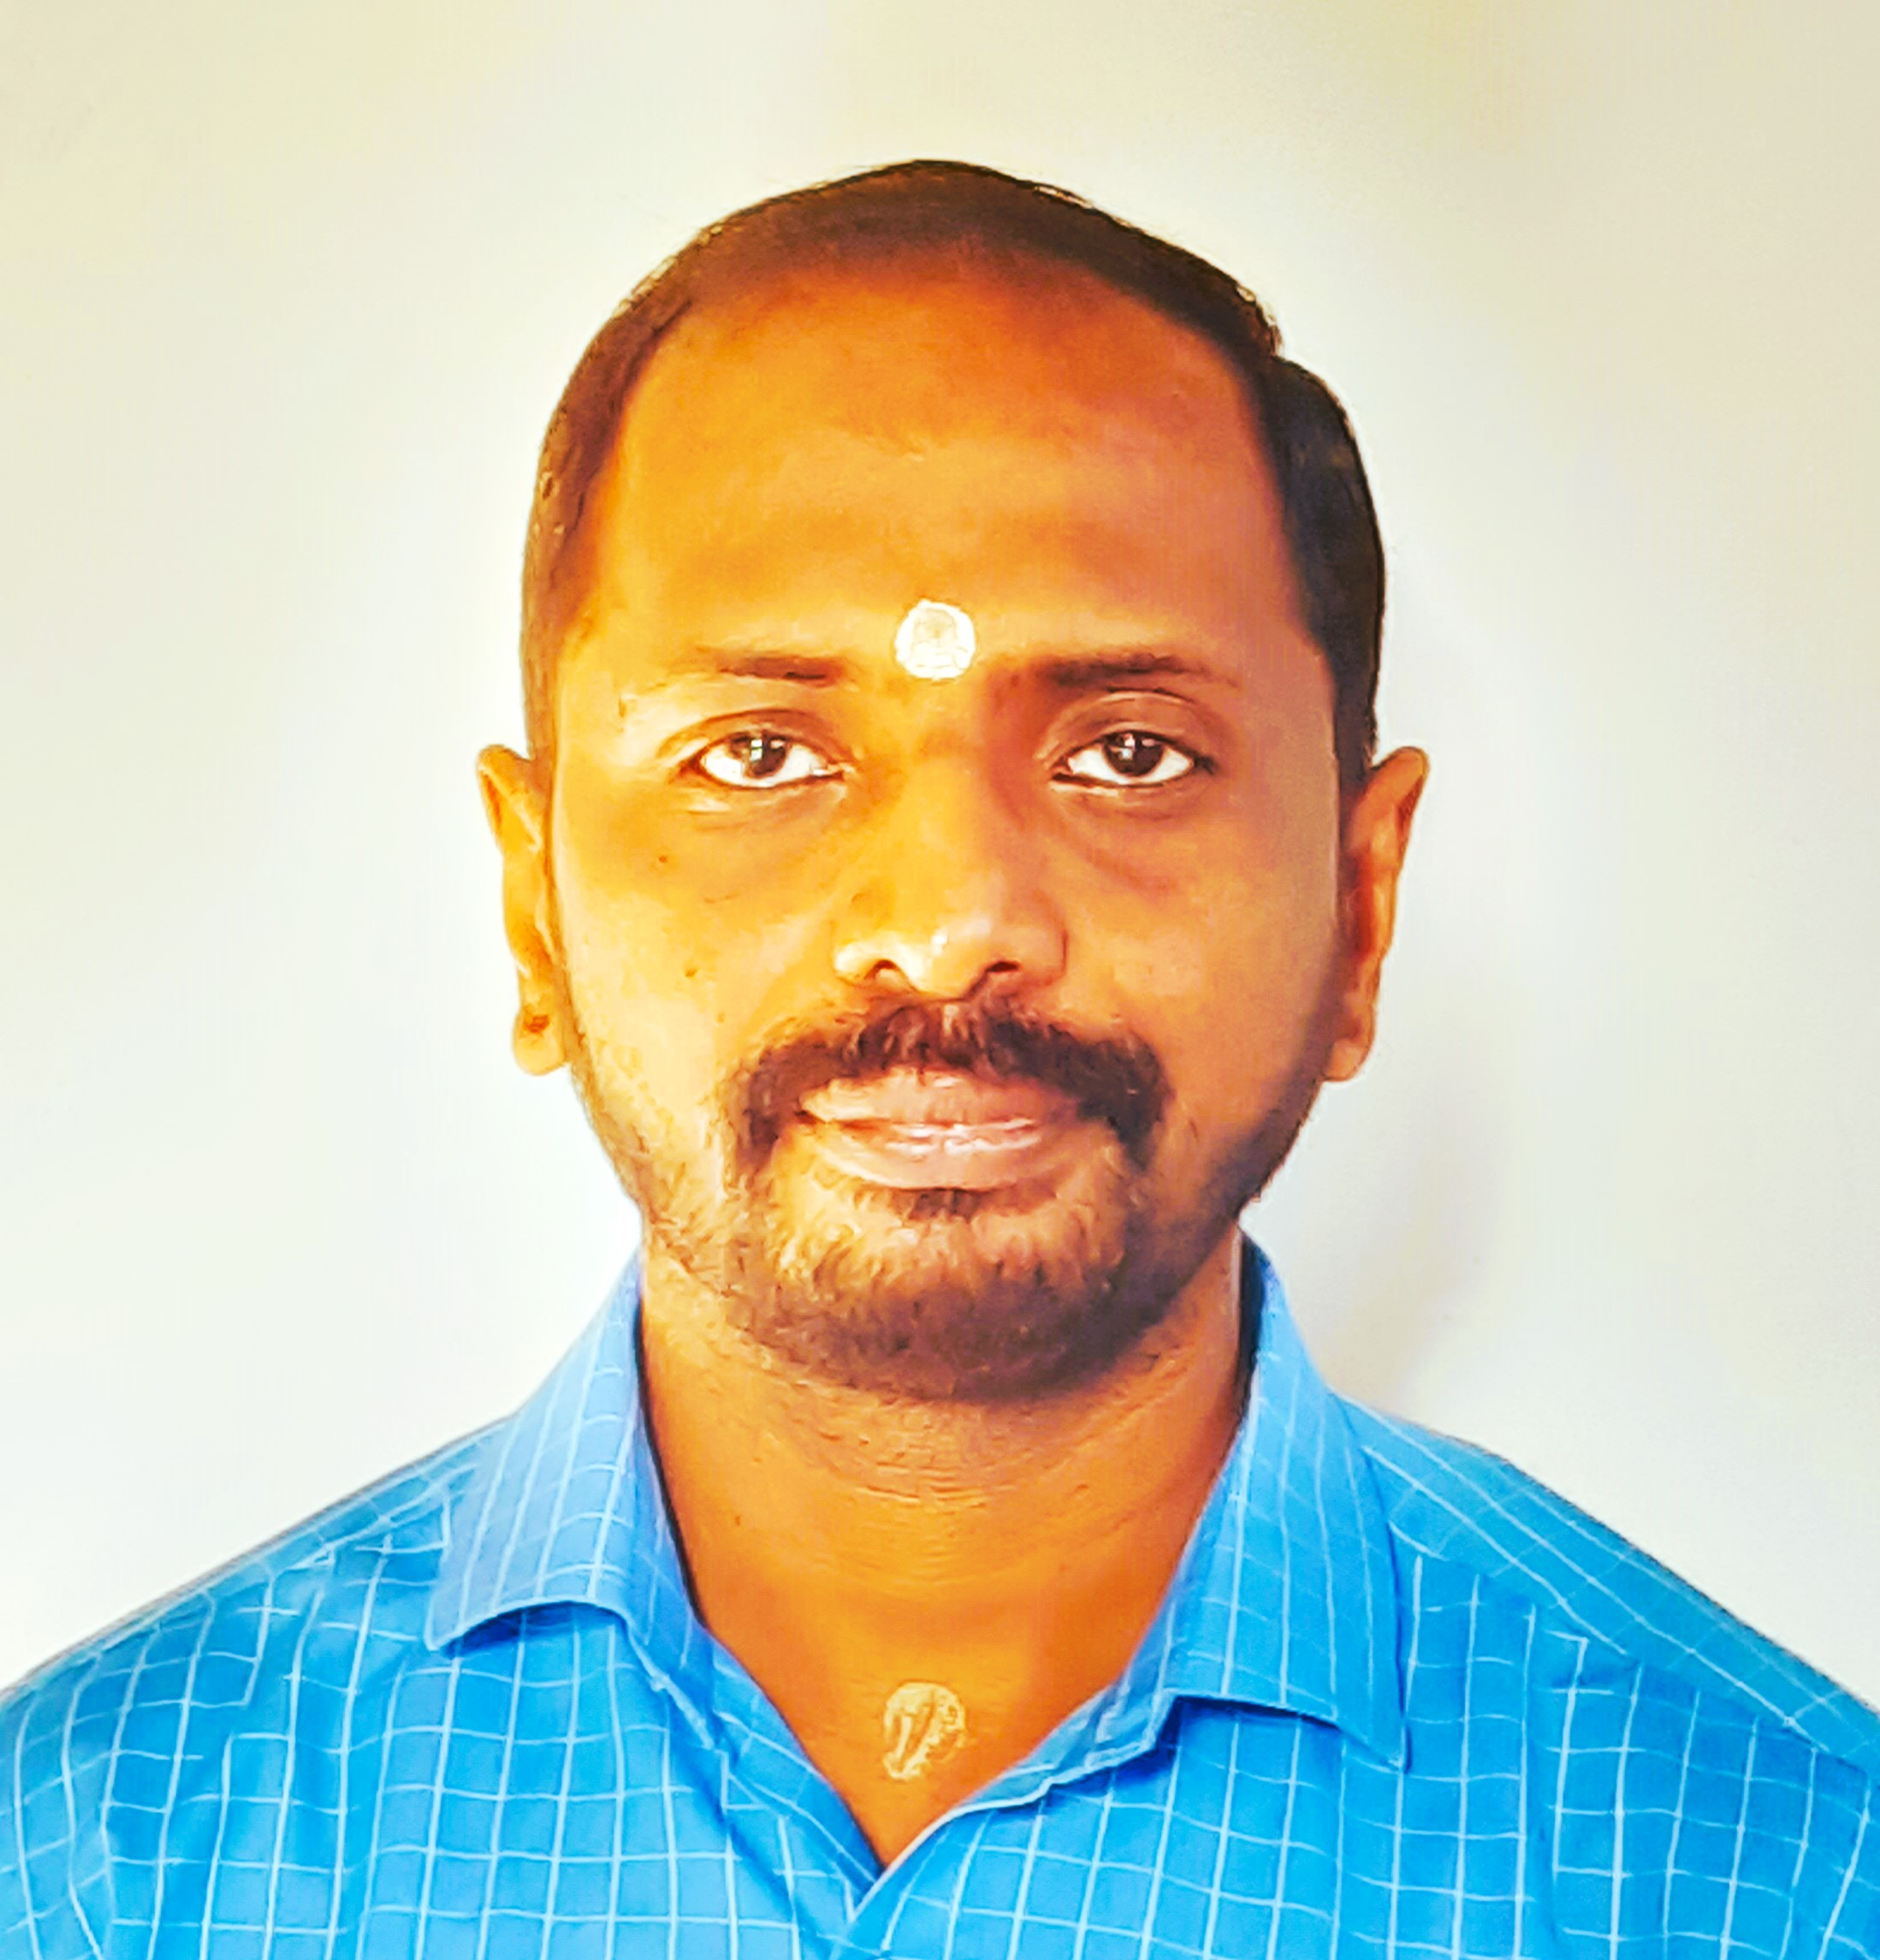
\includegraphics{Swamy.jpg}]{Siju K S}
true
\end{IEEEbiography}
\begin{IEEEbiography}[\includegraphics{soman\_sir.jpg}]{Dr.Soman K.P}
true
\end{IEEEbiography}
% that's all folks
\end{document}

